\documentclass[a4paper]{article}

\usepackage{microtype}
\usepackage{fullpage}
\usepackage{mathtools}
\usepackage{amsfonts}
\usepackage{tikz}
\usepackage{pgfplots}
\usepackage{hyperref}
\usepackage{amsthm}
\usepackage{xcolor}
\usepackage[noabbrev,nameinlink]{cleveref}
\usepackage{caption}
\usepackage{subcaption}
\usepackage{setspace}
\usepackage[backend=biber,style=authoryear,maxbibnames=99,hyperref=true]{biblatex}

\setstretch{1.15}

\addbibresource{src/paper/references.bib}

\usepgfplotslibrary{fillbetween}
\usetikzlibrary{shapes}
\pgfplotsset{compat=1.17}

\newtheorem{proposition}{Proposition}
\newtheorem{corollary}{Corollary}
\newtheorem{lemma}{Lemma}
\newtheorem{assumption}{Assumption}

\newcommand{\dt}{\mathrm{d}t}
\newcommand{\ds}{\mathrm{d}s}
\newcommand{\di}{\mathrm{d}i}
\newcommand{\dG}{\mathrm{d}G}
\newcommand{\E}{\mathbb{E}}
\newcommand{\Var}{\mathrm{Var}}

\DeclarePairedDelimiter\floor{\lfloor}{\rfloor}

\title{The value of being indispensable: a cooperative approach to bargaining with a continuum of players}
\author{Martin Stancsics}

\begin{document}

\maketitle

\begin{abstract}
    This paper investigates the idea of using concepts random order values, a concept from cooperative game theory, to model bargaining outcomes in games with an indispensable player and a continuum of fringe players.
    I show that this approach proves to be very tractable in a number of settings, and leads to results that are in line with one's intuitive expectations about bargaining outcomes.
    Thus, it can be a useful tool in modelling situations where one does not want to attribute all the bargaining power to one type of market participants, and at the same time would like to avoid having to deal with an explicit multi-stage bargaining game.
    On one hand, this paper provides a taxonomy of the various results found in some applied papers.
    Furthermore, it introduces some new results pertaining to the case when participants have different levels of innate bargaining power, and weighted values are more appropriate.
    The results in this paper is intended to be used as a tool-kit for embedding bargaining outcomes into more complex models.
\end{abstract}


\section{Motivation}

Using cooperative game theory to model bargaining outcomes in a tractable way has quite a few examples in the industrial organization literature.
This is in part motivated by the appealing properties of the resulting gain distributions, their tractability, but also by the long line of theoretical studies showing that various bargaining procedures lead to such outcomes.
For example, \textcite{gul1989bargaining,winter1994demand,hart1996bargaining,inderst2003bargaining,} or, perhaps most relevant to this paper, \textcite{stole1996intra} all propose various extensive-form bargaining games in which the expected outcomes correspond to players' Shapley-values.

In terms of applications, the case of one indispensable player and a large number of small ones is particularly important in a number of settings.
Examples include intra-firm ownership strutures \parencite{hart1990property}, wage bargaining \parencite{stole1996intra,stole1996organizational,levy1997individual}, collusion and mergers \parencite{segal2003collusion} and upstream-downstream supply chains \parencite{inderst2003bargaining,montez2007downstream}.
The study of multi-sided markets (paltforms) is also a good fit for this modeling approach, as the platform is often indispensable for the fringe firms, but the latter are also numerous enough to be approximated by a continuum.\footnote{
    \textcite{huang2022shapley} is one of the very few examples of using cooperative game theory in this setting.
}

A common feature of most of the aforementioned papers is that they assume a finite number of players.
However, as is often the case in economics, infinite-player approximations turn out to be more tractable while retaining the main conclusions of the finite models from which they arise.
Perhaps most importantly, the resulting profit shares become continuous and differentiable functions of the size of the fringe, which is particularly useful when embedding these results into more complex models.

Cooperative games with a finite number of atomic players and a continuum of non-atomic ones are called mixed or oceanic games \parencite{milnor1978values}, and have been studied in the literature of cooperative game theory.
Most papers in this line of research focus on questions such as for which games the Shapley-value exists and is unique \parencite{hart1973values}, and whether various approaches (namely, characterizing the value using a set of axioms, and taking the limit of the value of finite-player games) lead to the same result \parencite{fogelman1980asymptotic}.\footnote{
    \textcite{hart1973values} shows that in the case of mixed games, the usual axioms do not characterize a unique value in general.
    However, \textcite{fogelman1980asymptotic} demonstrates that, for a quite general subset of games, the asymptotic approach leads to one specific element from the set characterized by the axiomatic approach. 
}
My aim with this paper is both more general and more specific in certain aspects.
For one, I am only interested in the asymptotic approach, and withing that, a specific series of finite games.
Furthermore, I restrict my attention to one specific type of games, namely those with an indispensable player, and a continuum of fringe players consisting of a finite number of types.
This in turn allows me to go beyond the usual Shapley-value, and obtain results for a more general set of solution concepts: random order values.
A specific example of those, for which I provide a number of new results, is the weighted value \parencite{shapley1953additive}.
Additionally, due to more structure in the model, I am able to provide more concrete results, investigate some comparative statics, as well.

Despite their theoretical appeal and their tractability, oceanic games saw very little use in the industrial organization, and, more generally, applied economics literature.
The two most prominent examples are \textcite{stole1996intra, stole1996organizational} and \textcite{levy1997individual}, all of which use the Shapley-value to model wage bargaining, and consider the case of divisible labor (continuum of workers).
The first two of these paper also provides microfoundations for the Shapley value and the weighted value in the intra-firm bargaining setting.

In the following sections, I propose an oceanic game with the main feature that the large player is indispensable for creating value.\footnote{
    This assumption will be somewhat relaxed throughout some of the generalizations.
}
Such a model applies to all the settings mentioned above, such as intra-firm bargaining, vertical supply chains, or multi-sided markets.
I demonstrate that the Shapley values of the players in those models are described by very tractable expressions that have nice geometric interpretations.
Additionally, the outcomes are in line with one's intuitive expectations of bargaining power in such situations.
Finally, I demonstrate the usefulness of this approach by building a simple model of TODO.


\section{One-sided case}

In this section I examine the case of identical fringe players.
I will first look at the simplest setting (one large player, which is completely indispensable), but in the subsequent sections I will somewhat relax this assumption.
Let us start by defining the cooperative game that describes this situation.

Consider a game with two types of players: a major player $P$ and $n$ smaller players $A_i$, $1 \leq i \leq n$.
Formally, let us denote the set of all players as $N = \{P, A_1, \dots, A_n\}$.
Assume that (1) no coalition of players can achieve a positive value without the participation of $P$ and (2) players $A_i$ are identical.
Let $n_T(S)$ denote the number of players of type $T \in \{P, A\}$ in coalition $S$.
Under these assumptions, the characteristic function of the game (the value that any coalition $S \subset N$ can achieve) is the following:
\begin{align*}
    v(S) = \begin{cases}
        0                              & \text{if } P \notin S \\
        f\left(\frac{n_A(S)}{n}\right) & \text{otherwise}.
    \end{cases}
\end{align*}
One can think of this setting as a (one-sided) platform and a number of potential entrants, if the entrants can only reach their prospective consumers through the platform, or as a vertical supply chain with one upstream producer and a number of downstream firms.

First, let us characterize the conditions under which this game is monotone and superadditive.
Superadditivity is a key property of cooperative games, as it ensures that it always pays off to form the grand coalition (i.e., the coalition that includes all players).
Furthermore, in the context of bargaining, these properties provide some theoretical support for using Shapley-values as bargaining outcomes, as many results creating a link between non-cooperative bargaining and cooperative values often rely on these assumptions.\footnote{
    For example, the results in \textcite{gul1989bargaining} rely on superadditivity, while monotonicity suffices for \textcite[]{hart1996bargaining}.
}
In this specific setting, characterizing monotonicity and superadditivity is extremely straightforward.
\begin{proposition}
    \label{prop:monotone}
    The game $(N, v)$ is monotone and superadditive if and only if $f$ is increasing and $f(0) \geq 0$.
\end{proposition}

In the following, let us assume that the assumptions required for monotonicity are always satisfied (i.e., $f$ is monotone increasing).\footnote{
    This assumption is not entirely innocuous.
    For example, having more small firms could in theory lead to stronger competition, decreasing total profits.
    However, it often holds in models with network effects \parencite{rochet2003platform} or with consumers having taste for variety \parencite{anderson2020aggregative}.
}
As a side note, it also ensures that the games are of bounded variation, and thus the main theorem in \textcite{fogelman1980asymptotic} applies.
Namely, both the asymptotic and axiomatic approach of characterizing the Shapley-value of the game lead to the same result\footnote{
    More precisely, the asymptotic value coincides with the axiomatic one derived using the uniform distribution.
    For a more detailed discussion, see \textcite{fogelman1980asymptotic}.
}.

\subsection{Random order values}

For any finite number of fringe players, the random order value of a player \parencite{weber1988probabilistic} is simply its average marginal contribution to the value of all possible coalitions.
More precisely, take all permutations of the players, and assign a probability to each of them.
Then, the random order value of player $P$ is the expected marginal contribution of $P$ to the value of the coalition preceding it in these permutations.

For the remainder of the paper, let us use the following notation: $\varphi_P^n$ denotes the (depending on section, Shapley, weighted or random order) value of player $P$ in the game with players $N = \{P, A_1, \dots, A_n\}$.
Then, formally,
\begin{align*}
    \varphi_P^n = \frac{1}{(n+1)!} \sum_{R} \Pr(R) [ v(\mathcal{P}_P^R \cup \{i\}) - v(\mathcal{P}_P^R) ]
\end{align*}
where $R$ is a permutation of all players, and $\mathcal{P}_P^R$ is the set of players before $P$ in the permutation $R$. \footnote{
    For example, if $R = \{A_1, P, A_2\}$, then $\mathcal{P}_P^R = \{A_1\}$.
}

Random order values are of interest to us for a number of reasons.
First, they are a natural extension to the Shapley value, where the axiom of symmetry is relaxed.
Furthermore, they provide a convenient framework, of which all subsequent results (Shapley value, weighted value, multiple big players) are special cases.

Utilizing the fact that the value of any coalition is zero without $P$, and that -- conditional on player $P$ being in a coalition -- a coalition's value only depends on the number of fringe firms in it, the above expression can be simplified to the following:
\begin{align*}
    \varphi_P^n = \frac{1}{n+1} \sum_{k=0}^n \Pr(|\mathcal{P}_P| = k) f(k/n),
\end{align*}
where $\Pr(|\mathcal{P}_P| = k)$ is determined by the probability distribution over the permutations.

Now let us look at the asymptotic limit of this expression, as the number of fringe players goes to infinity.
The following proposition demonstrates the main idea of this paper: even as the number of fringe players goes to infinity, the value of the big player does not converge to the worth of the grand coalition, $f(1)$.

\begin{proposition}
    \label{prop:one_sided_general}
    Let $f$ be continuous on [0, 1]. Furthermore, let us denote the random variable $\frac{|\mathcal{P}_P|}{n}$ as $X_n$. Assume that $X_n \xrightarrow[]{d} X$ with cdf $G_X(t)$ and (if exists) pdf $g(t)$.
    Then
    \begin{align*}
        \varphi_P^\infty = \lim_{n \to \infty} \varphi_P^n = \int_0^1 f(t) \dG(t) = \int_0^1 g(t) f(t) \dt,
    \end{align*}
    with the last equality holding if $X$ is a continuous random variable.
\end{proposition}

Now let us turn to the value of the fringe.
The following corollary shows that the aggregated value of the fringe remains positive even in the limit.
In other words, even though the fringe players become smaller and more numerous, they do not lose all of their bargaining power, and still end up with a positive payoff in the end.
\begin{corollary}
    \label{cor:fringe_value_general}
    The aggregated value of the fringe is
    \begin{align*}
        \varphi_A^\infty = f(1) - \int_0^1 f(t) \dG(t).
    \end{align*}
    Furthermore, if $f$ is differentiable on $[0, 1]$, then the value of the fringe can also be expressed as
    \begin{align*}
        \varphi_A^\infty = \int_0^1 G(t) f'(t) \dt.
    \end{align*}
\end{corollary}

It also provides us with two ways of thinking about the value of the fringe.
First, due to random order values being efficient, it can be thought of as the leftover from the total value after subtracting the value of the big player.
Alternatively, as the second part of the corollary demonstrates, it is also related to the marginal contributions to the fringe agents.
The only difference from the big player's value is that we have to weight this marginal contribution by the probability of the big player appearing before the fringe firm in question, as otherwise its marginal contribution is zero.
The latter interpretation will be particularly useful when thinking about the value of the fringe in the multi-sided setting.

It is immediately follows from the proposition above that (for a fixed total pie size $f(1)$) player $P$ gets a larger share when $f(t)$ is larger for every $t$.
It is already apparent from Figure \ref{fig:one_sided} that (for a fixed total pie size $f(1)$) player $P$ gets a larger share when $f(t)$ is larger for every $t$.
It corresponds to the case when only a relatively small fraction of the fringe is needed to create a large part of the total potential surplus (e.g. fringe players products are substitutes of each other).
This result aligns with our natural intuition that player $P$ has a better bargaining position in this case, than if only coalitions with most of the fringe firms on board could obtain high values.
In contrast, when fringe players are more complementary to each other, the big player can only obtain a smaller share, as its bargaining power is more limited.


\subsection{Shapley value}

Now let us turn our attention to an important special case of random order values: the Shapley value.
It can be characterized by being the random order value that additionally also satisfies the axiom of symmetry.
This axiom requires that if two players are identical in terms of the characteristic function, then they should receive the same value.
Equivalently, it is the same as requiring that all permutations have an equal probability.

The following proposition and corollary derives the Shapley value of the big player and the fringe, respectively.

\begin{proposition}
    \label{prop:one_sided}
    Let $f$ be continuous on [0, 1]. Then
    \begin{align*}
        \varphi_P^\infty = \lim_{n \to \infty} \varphi_P^n = \int_0^1 f(t) \dt .
    \end{align*}
\end{proposition}

\begin{corollary}
    \label{cor:fringe_value}
    The aggregated Shapley-value of the fringe is
    \begin{align*}
        \varphi_A^\infty = f(1) - \int_0^1 f(t) \dt.
    \end{align*}
    Furthermore, if $f$ is differentiable on $[0, 1]$, then the value of the fringe can also be expressed as
    \begin{align*}
        \varphi_A^\infty = \int_0^1 t f'(t) \dt.
    \end{align*}
\end{corollary}

Because the Shapley value is a special case of the random order value, these results follows quite straightforwardly from \cref{prop:one_sided_general} and \cref{cor:fringe_value_general}.
One only has to notice that each permutation having an equal probability implies that the number of firms coming before $P$ is uniformly distributed on $1, \dots, n$, and thus the share of firms before $P$ converges in distribution to the uniform distribution on $[0, 1]$.
Alternatively, a more direct proof is provided in \cref{sec:proofs}, or a probabilistic justification can be found in \textcite{levy1997individual}.

The resulting Shapley values also have a nice geometric interpretation \cref{fig:one_sided}.
Consider a rectangle with sides of length 1 and $f(1)$, respectively.
Then, due to superadditivity, the grand coalition forms and achieves the value $f(1)$, which is the area of the rectangle.
The value of the big player is then $\int_0^1 f(t) \dt$, which is simply the part of the rectangle below the graph of $f$, while the fringe gets the rest.
Thus, the graph of $f$ partitions the area (total value) into what the big player and the fringe obtain.

\begin{figure}
    \centering
    \begin{subfigure}[b]{0.45\textwidth}
        \centering
        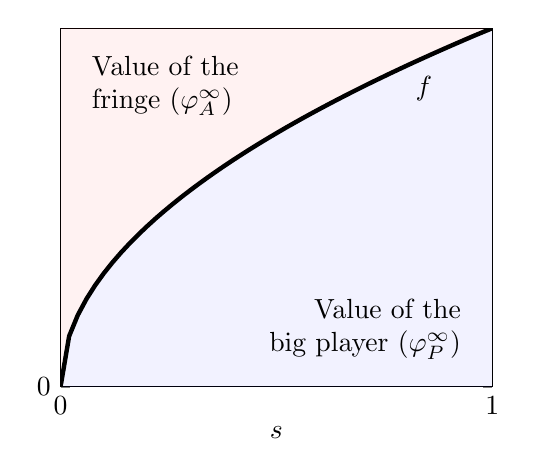
\begin{tikzpicture}[scale=0.8]
            \begin{axis}[xmin=0, xmax=1, ymin=0, ymax=1, samples at={0, 0.02, ..., 0.98, 1},
                    xtick={0, 1}, ytick={0}, xlabel={$s$}]
                \addplot[name path=f, ultra thick] {x^0.5};
                \node[anchor=north west] at (axis cs: .8, .8^0.5) {$f$};
                \path[name path=bottom] (axis cs:0,0) -- (axis cs:1,0);
                \path[name path=top] (axis cs:0,1) -- (axis cs:1,1);

                \addplot [fill=blue, fill opacity=0.05] fill between [of=f and bottom];
                \addplot [fill=red, fill opacity=0.05] fill between [of=f and top];

                \node[anchor=north west, align=left] at (axis cs: .05, .95) {Value of the \\ fringe ($\varphi_A^\infty$)};
                \node[anchor=south east, align=right] at (axis cs: .95, .05) {Value of the \\ big player ($\varphi_P^\infty$)};
            \end{axis}
        \end{tikzpicture}
        \caption{Fringe players are each other's substitutes}
    \end{subfigure}
    \begin{subfigure}[b]{0.45\textwidth}
        \centering
        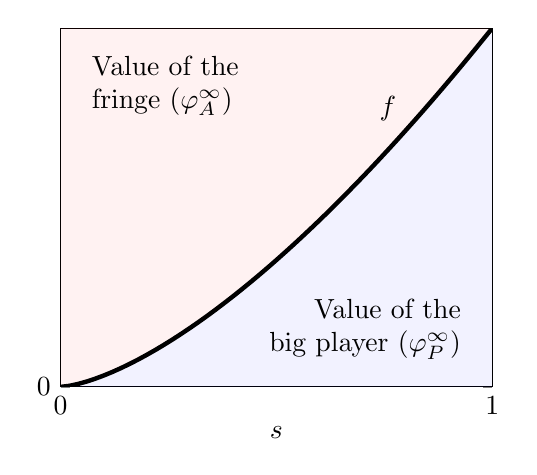
\begin{tikzpicture}[scale=0.8]
            \begin{axis}[xmin=0, xmax=1, ymin=0, ymax=1, samples at={0, 0.02, ..., 0.98, 1},
                    xtick={0, 1}, ytick={0}, xlabel={$s$}]
                \addplot[name path=f, ultra thick] {x^1.5};
                \node[anchor=south east] at (axis cs: .8, .8^1.5) {$f$};
                \path[name path=bottom] (axis cs:0,0) -- (axis cs:1,0);
                \path[name path=top] (axis cs:0,1) -- (axis cs:1,1);

                \addplot [fill=blue, fill opacity=0.05] fill between [of=f and bottom];
                \addplot [fill=red, fill opacity=0.05] fill between [of=f and top];

                \node[anchor=north west, align=left] at (axis cs: .05, .95) {Value of the \\ fringe ($\varphi_A^\infty$)};
                \node[anchor=south east, align=right] at (axis cs: .95, .05) {Value of the \\ big player ($\varphi_P^\infty$)};
            \end{axis}
        \end{tikzpicture}
        \caption{Fringe players are each other's complements}
    \end{subfigure}
    \caption{Distribution of value between player $P$ (red) and the fringe (blue)}
    \label{fig:one_sided}
\end{figure}

Finally, the following corollary highlights that, even though the individual share of each $A_i$ vanishes as their number goes to infinity, their total value still remains positive.
\begin{corollary}
    \label{cor:fringe_value_2}
    $\varphi_P^\infty < f(1)$ and $\varphi_A^\infty > 0$ for any $f$ that is not constant.
\end{corollary}


\paragraph{Example: power function.}

Let us illustrate the results of this section with a simple example.
Consider the case when $f(n) = n^\alpha$, for some $\alpha > 0$.
Assume that the bargaining takes place between player $P$ and a measure $\bar{n}$ of fringe players.
Thus, the value that the grand coalition can achieve is $\bar{n}^\alpha$.

\Cref{prop:many_sided_shapley} shows that the value of player $P$ in this case is
\begin{align*}
    \varphi_P^\infty(\bar{n}) = \int_0^1 (s \bar{n})^\alpha = \frac{1}{\alpha + 1} \bar{n}^\alpha,
\end{align*}
while the fringe gets the rest, i.e.,
\begin{align*}
    \varphi_A^\infty(\bar{n}) = \bar{n}^\alpha - \frac{1}{\alpha + 1} \bar{n}^\alpha = \frac{\alpha}{\alpha + 1} \bar{n}^\alpha.
\end{align*}

In words, regardless of the value of $\bar{n}$, the two types of players share the total value in the same proportion.
This proportion depends on the parameter $\alpha$ (\cref{fig:power_function_example}), which can be interpreted as the degree of substitutability between the fringe players.
More specifically, the higher $\alpha$ is, the more complementary the fringe players are to each other, and the larger the share they obtain.
In the limit, when $\alpha \to \infty$, the fringe obtains all the value, as essentially all players become indispensable, and share the total value equally.
On the other hand, when $\alpha \to 0$, the big players can appropriate all the value.

\begin{figure}
    \centering
    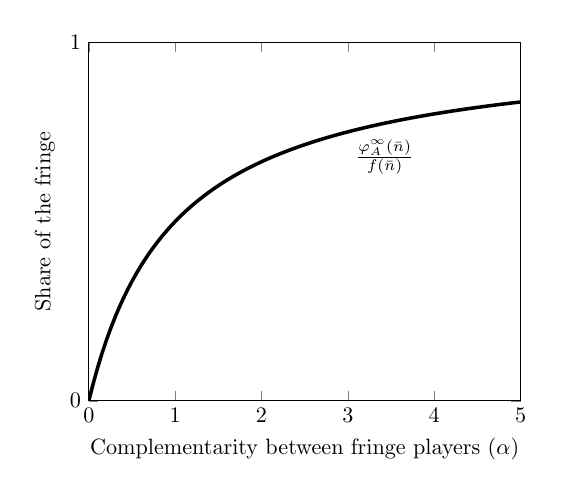
\begin{tikzpicture}[scale=0.8]
        \begin{axis}[xmin=0, xmax=5, ymin=0, ymax=1, samples at={0, 0.05, ..., 4.95, 5},
                xtick={0, 1, 2, 3, 4, 5}, ytick={0, 1},
                xlabel={Complementarity between fringe players ($\alpha$)}, ylabel={Share of the fringe}]
            \addplot[name path=f, ultra thick] {x / (1 + x)};
            \node[anchor=north west] at (axis cs: 3, 3/4) {$\frac{\varphi_A^\infty(\bar{n})}{f(\bar{n})}$};
            \path[name path=bottom] (axis cs:0,0) -- (axis cs:1,0);
            \path[name path=top] (axis cs:0,1) -- (axis cs:1,1);
        \end{axis}
    \end{tikzpicture}
    \caption{Example: share of the fringe as a function of $\alpha$ (degree of complementarity between fringe players)}
    \label{fig:power_function_example}
\end{figure}


\subsection{Weighted values}

This section investigates the case when players have different levels of innate bargaining power.
One way to model this is by using weighted values \parencite{shapley1953additive}, which are a generalization of the Shapley value.
The idea behind them is that, in addition to the set of players and the characteristic function, the game is also endowed with a weight system, which is a vector of non-negative numbers, one for each player.
These weights determine how the value of a coalition is distributed amongst its members in the case when they are all equally important for the coalition.
This is a way to relax the symmetry axiom of Shapley values, while retaining more structure than in the case of the more general random order values.

These weights can be thought of as the measure of some innate bargaining power, not reflected in the value function.\footnote{
    Although, this interpretation is not always appropriate.
    As \textcite{owen1968communications} demonstrates, there are games where the weighted value is not monotone increasing in a player's weight.
}
Further support for this interpretation in certain games can be found in \textcite{hart1996bargaining}, demonstrating that in a certain alternating offer bargaining game, weights are related to the probability of each player making the offer.\footnote{
    For example, only one player having a positive value corresponds to them making take it or leave it offers.
}
Additionally, \textcite{stole1996intra} provides an alternative microfoundation for the weighted value in the case of non-binding contracts.

For my purposes, it is sufficient to deal with the case of simple weights.
I.e., assume that there is at most one player with zero weight.
For my main result, I make use of the fact that weighted values can be calculated by weighting the permutations by the probabilities arising from the following sequential ordering procedure \parencite{kalai1987weighted}.
Start with the set of all players.
Let the probability of player $i$ being the last amongst the set of remaining players $R$ be $\lambda_i / \sum_{j \in R} \lambda_j$.
Continue until all players are exhausted.
This yields a well-defined probability for each permutation of players.

Consider the game described in the previous section, and let the weights of players of type $A$ and $P$ be 1 and $\lambda$, respectively.
Let $X_n$ be a random variable representing the number of players before $P$ when players are ordered according to the previously described procedure.
Then, the probability of player $P$ having at most $k$ players of type $A$ before themselves is simply
\begin{align}
    \label{eq:entry_distr_discrete}
    \Pr(X_n \leq k) = \prod_{j=k+1}^n \frac{j}{j + \lambda}.
\end{align}
The following lemma establishes the continuous analogue of this statement.
\begin{lemma}
    \label{lem:entry_distr}
     As $n \to \infty$, $X_n \xrightarrow[]{d} X$ with the cdf $G_X(t) = \lambda^t$.
     Consequently, the corresponding probability density function is $g(t) = \lambda t^{\lambda - 1}$.
\end{lemma}

Now we have everything we need to derive the weighted value of both types of players.
Having \cref{eq:entry_distr_discrete} and \cref{lem:entry_distr} allows us to invoke \cref{prop:one_sided_general} to obtain the following proposition.\footnote{
    \textcite{stole1996intra} also derives essentially the same expression for the equilibrium outcome of their bargaining game with unequal profit distribution, and assert that it is equal to the weighted value.
}

\begin{proposition}
    \label{prop:one_sided_weighted}
    Let $f(t)$ be continuous on $[0, 1]$. Then
    \begin{align*}
        \varphi_P(\lambda, \infty) = \int_0^1 g(t) f(t) \dt
    \end{align*}
    where $g(t) = \lambda t^{\lambda - 1}$.

    Furthermore,
    \begin{align*}
        \varphi_A(\lambda, \infty) &= 1 - \int_0^1 g(t) f(t) \dt \\
                                   &= \int_0^1 G(t) f'(t) \dt,
    \end{align*}
    where $G(t) = t^\lambda$.
\end{proposition}

Depending on the shape of this distribution (which in turn depends on the weight $\lambda$), regions corresponding to different masses of fringe firms can be over or underweighted in this integral, leading to different values.

\begin{figure}[ht]
    \centering
    \begin{subfigure}[b]{0.45\textwidth}
        \centering
        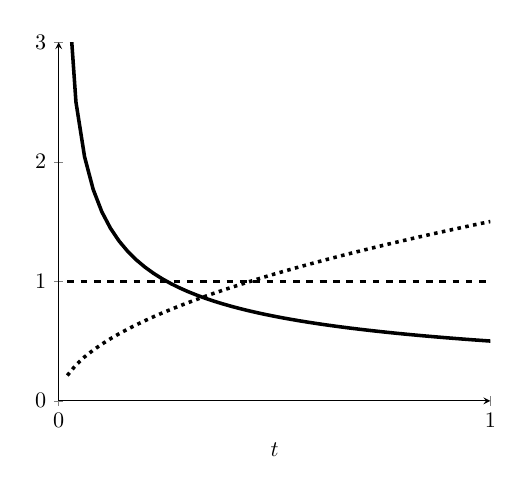
\begin{tikzpicture}[scale=0.8]
            \begin{axis}[xmin=0, xmax=1, ymin=0, ymax=3, samples at={0.02, 0.04, ..., 0.98, 1},
                xtick={0, 1}, ytick={0, 1, 2, 3}, axis lines=left, xlabel={$t$}, legend pos=south east]
                \addplot[ultra thick] {0.5 * x ^ (-0.5)};
                \addplot[ultra thick, dashed] {1};
                \addplot[ultra thick, dotted] {1.5 * x ^ (0.5)};
            \end{axis}
        \end{tikzpicture}
        \caption{$g(t)$}
    \end{subfigure}
    \begin{subfigure}[b]{0.45\textwidth}
        \centering
        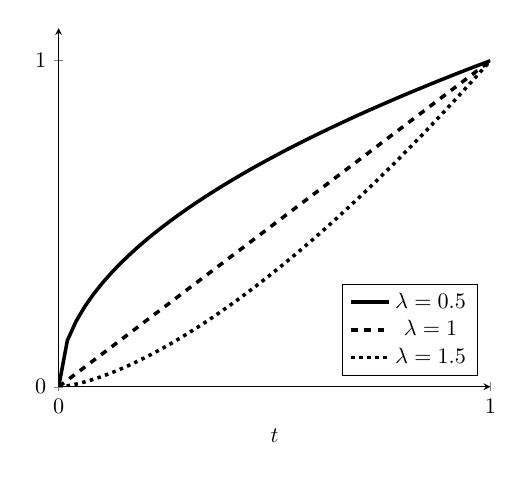
\begin{tikzpicture}[scale=0.8]
            \begin{axis}[xmin=0, xmax=1, ymin=0, ymax=1.1, samples at={0, 0.02, ..., 0.98, 1},
                xtick={0, 1}, ytick={0, 1}, axis lines=left, xlabel={$t$}, legend pos=south east]
                \addplot[ultra thick] {x ^ (0.5)};
                \addplot[ultra thick, dashed] {x};
                \addplot[ultra thick, dotted] {x ^ (1.5)};
                \legend{$\lambda = 0.5$, $\lambda = 1$, $\lambda = 1.5$}
            \end{axis}
        \end{tikzpicture}
        \caption{$\int_0^t g(s) \ds$}
    \end{subfigure}
    \caption{Illustration of the weighting function for various values of $\lambda$ in the weighted Shapley-value.}
    \label{fig:weigh_function}
\end{figure}

Now, let us examine how this weighting impacts the shares of the various players.
It turns out, that a higher weight corresponds to a higher Shapley-value in this game.\footnote{
    This would not necessarily have to be the case, as demonstrated by \textcite{owen1968communications}.
},
supporting the interpretation of weights as some kind of innate bargaining power.
\begin{corollary}
    \label{cor:platform_value_weighted}
    $\varphi_P(\lambda, \infty)$ is increasing in $\lambda$ unless $f$ is constant.
\end{corollary}

Furthermore, the following corollary shows that the limit of the weighted value of $P$, as their weight goes to zero (infinity) is precisely the payoffs $P$ would achieve if $P$ were making (facing) take-it-or-leave-it offers.
This set of results highlights that utilizing (weighted) Shapley values to model bargaining outcomes provides an intermediate solution between inscribing all the bargaining power to one or the other player.
\begin{corollary}
    \label{cor:paltform_value_weighted_2}
    If the weight of player $P$ goes to infinity (zero), its weighted Shapley value converges to $f(1)$ ($f(0)$).
\end{corollary}

\subsection{Shapley value with multiple big players}

Now imagine that, instead of just one, there are $m$ players of type $P$, and they are perfect substitutes of each other.
That is, the fringe players still need one at least of them to achieve any value, but it does not matter which and how many of them are present.
Formally, the value function for coalition $S$ becomes the following:
\begin{align*}
    v(S) = \begin{cases}
        0                              & \text{if } n_P(S) = 0 \\
        f\left(\frac{n_A(S)}{n}\right) & \text{otherwise}.
    \end{cases}
\end{align*}

Let us start by establishing monotonicity for this version of the model, too.
\begin{proposition}
    The game is monotone if $f$ is increasing and $f(0) \geq 0$.
\end{proposition}
On the other hand, superadditivity is not as simple in this case, as before.
For example, when $f$ is concave, then $m$ coalitions with one platform each and the fringe divided equally amongst them clearly achieve a higher total payoff than the grand coalition.
Therefore, the results of this section are most applicable to settings when multiple coalitions cannot be formed at the same time for some reason.
For example, \textcite{hart1996bargaining} propose an interpretation when there is a single, indivisible, non-replicable resource or technology (not captured in the value function) necessary to produce any value.

As before, the main proposition in this section provides us with an expression of the limit of the value for this variant of the game.
Notably, as in the case of the weighted value, the share of player $P$ can again be expressed as an integral of $f$ and some weighting\footnote{
    Weighting is not a completely precise term, as $h(t)$ does not integrate to one, and is therefore not a probability distribution in this case (\cref{fig:multiple_platforms}).
} function $h(t)$, with the latter depending only on the number of big players.
\begin{proposition}
    \label{prop:multiple_platforms}
    The limit of the Shapley-value (as $n \to \infty$) of each player of type $P$ is
    \begin{align*}
        \varphi_{P_i}^{\infty, m} = \int_0^1 h(t) f(t) \dt,
    \end{align*}
    where $h(t) = (1-t) ^ {m-1}$.
\end{proposition}

As with proposition \ref{prop:one_sided}, this result also has a probabilistic interpretation.
Let the location of the $m$ atoms be $t_1, \dots, t_m$, distributed independently and uniformly on the unit interval.
The expected marginal contribution of $t_i$ is only positive whenever it is the first amongst the major players.
That is, for any $t_i$, the probability if $P_i$ being the first is related to the cdf of the first order statistic from $n-1$ independent uniform distributions: $1 - (1-t)^{m-1}$.

\begin{figure}[ht]
    \centering
    \begin{subfigure}[b]{0.45\textwidth}
        \centering
        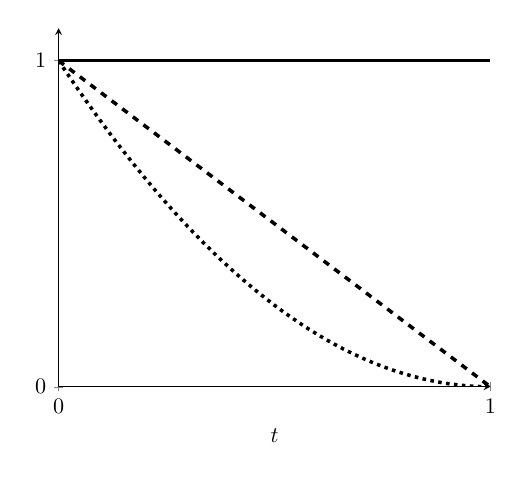
\begin{tikzpicture}[scale=0.8]
            \begin{axis}[xmin=0, xmax=1, ymin=0, ymax=1.1, samples at={0, 0.02, 0.04, ..., 0.98, 1},
                xtick={0, 1}, ytick={0, 1}, axis lines=left, xlabel={$t$}, legend pos=north west]
                \addplot[ultra thick] {1};
                \addplot[ultra thick, dashed] {1-x};
                \addplot[ultra thick, dotted] {(1-x)^2};
            \end{axis}
        \end{tikzpicture}
        \caption{$h(t)$}
    \end{subfigure}
    \begin{subfigure}[b]{0.45\textwidth}
        \centering
        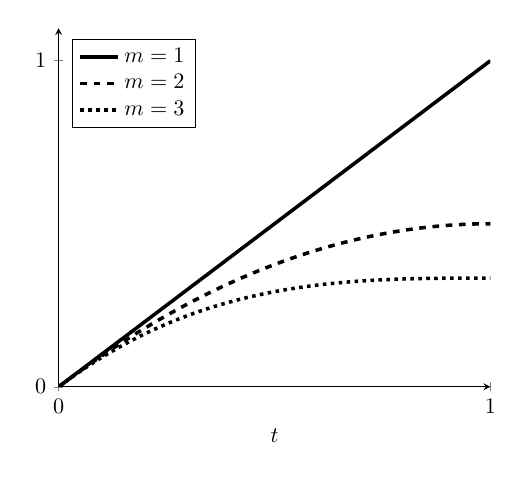
\begin{tikzpicture}[scale=0.8]
            \begin{axis}[xmin=0, xmax=1, ymin=0, ymax=1.1, samples at={0, 0.02, ..., 0.98, 1},
                xtick={0, 1}, ytick={0, 1}, axis lines=left, xlabel={$t$}, legend pos=north west]
                \addplot[ultra thick] {x};
                \addplot[ultra thick, dashed] {x - x^2/2};
                \addplot[ultra thick, dotted] {x - x^2 + x^3/3};
                \legend{$m = 1$, $m = 2$, $m = 3$}
            \end{axis}
        \end{tikzpicture}
        \caption{$\int_0^t h(s) \ds$}
    \end{subfigure}
    \caption{Illustration of the weighting function for various values of $m$ in the multiple big player case -- individual big player.}
    \label{fig:multiple_platforms}
\end{figure}

Let us examine the total value of all the big players.
Denote the aggregated value of players of type $P$ as $\varphi_{P}^{\infty, m} \coloneqq \sum_{j=1}^m\varphi_{P_j}^{\infty, m} = m\varphi_{P_i}^{\infty, m}$.
It immediately follows from the previous proposition that
\begin{align*}
    \varphi_{P}^{\infty, m} = \int_0^1 g(t) f(t) \dt,
\end{align*}
where $g(t) = m (1-t) ^ {m-1}$.
Notice that $g(t)$ now integrates to one, and is thus a probability distribution (\cref{fig:multiple_platforms_total}).
Therefore, the Shapley value in the case of multiple, substitutable big players can be interpreted as a random order value with a single big player.
The probability distribution for the corresponding random order value has a specific form, and its only parameter is the number of big players.
Thus, all the results from the previous section apply to this case as well.

\begin{figure}[ht]
    \centering
    \begin{subfigure}[b]{0.45\textwidth}
        \centering
        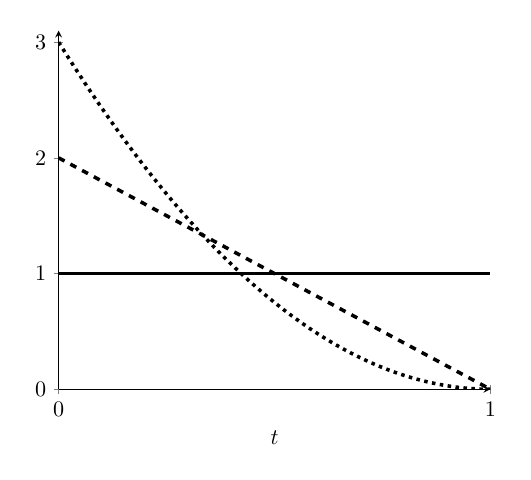
\begin{tikzpicture}[scale=0.8]
            \begin{axis}[xmin=0, xmax=1, ymin=0, ymax=3.1, samples at={0, 0.02, 0.04, ..., 0.98, 1},
                xtick={0, 1}, ytick={0, 1, 2, 3}, axis lines=left, xlabel={$t$}, legend pos=north west]
                \addplot[ultra thick] {1};
                \addplot[ultra thick, dashed] {2 * (1-x)};
                \addplot[ultra thick, dotted] {3 * ((1-x)^2)};
            \end{axis}
        \end{tikzpicture}
        \caption{$g(t)$}
    \end{subfigure}
    \begin{subfigure}[b]{0.45\textwidth}
        \centering
        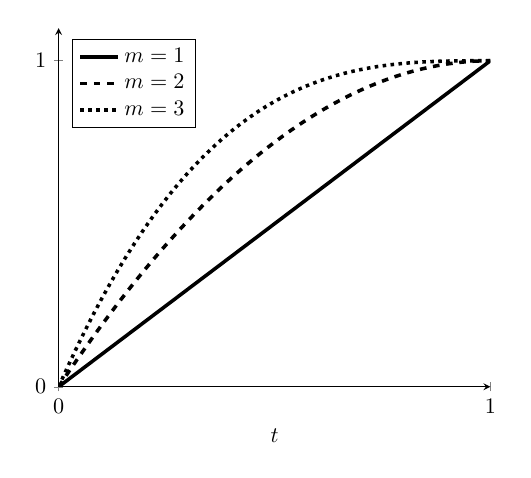
\begin{tikzpicture}[scale=0.8]
            \begin{axis}[xmin=0, xmax=1, ymin=0, ymax=1.1, samples at={0, 0.02, ..., 0.98, 1},
                xtick={0, 1}, ytick={0, 1}, axis lines=left, xlabel={$t$}, legend pos=north west]
                \addplot[ultra thick] {x};
                \addplot[ultra thick, dashed] {2 * (x - x^2/2)};
                \addplot[ultra thick, dotted] {3 * (x - x^2 + x^3/3)};
                \legend{$m = 1$, $m = 2$, $m = 3$}
            \end{axis}
        \end{tikzpicture}
        \caption{$\int_0^t g(s) \ds$}
    \end{subfigure}
    \caption{Illustration of the weighting function for various values of $m$ in the multiple big player case -- total of big players.}
    \label{fig:multiple_platforms_total}
\end{figure}

Now let us look at how the value of the big players and the fringe changes as a function of the number of the big players.
Proposition \cref{cor:multiple_platforms_2} again confirms our intuition: more players means that they become more substitutable, and thus their bargaining power decreases.
This not only means that the value of each individual big player decreases, but also that their total value goes down.

\begin{corollary}
    \label{cor:multiple_platforms_2}
    Let $\varphi_{P}^{\infty, m} = m\varphi_{P_i}^{\infty, m}$ denote the aggregated values of players of type $P$. $\varphi_{P}^{\infty, m}$ is decreasing in $m$ and $\varphi_{A}^{\infty, m}$ is increasing in $m$ unless $f$ is constant.
\end{corollary}

Finally, let us show that the value of the fringe has a similar, marginal contribution-based interpretation as in the case of a single big player.

\begin{corollary}
    \label{cor:multiple_platforms}
    The per-unit Shapley-value of the fringe is
    \begin{align*}
        \varphi_A^{\infty, m} = 1 - \int_0^1 f(t) \dG(t) = \int_0^1 G(t) f'(t) \dt ,
    \end{align*}
    where $G(t) = 1 - (1-t)^m$.
\end{corollary}


\subsection{Non-indispensable big player}

As a final extension for the one-sided case, let us examine what happens when the big player is not indispensable.
Assume that it provides some value to any coalition, but a coalition of fringe players can achieve a positive value without it.
Formally, the value function is the following:
\begin{align*}
    v(S) = \begin{cases}
        f_0\left(\frac{n_A(S)}{n}\right) & P \notin S \\
        f\left(\frac{n_A(S)}{n}\right)   & \text{otherwise}.
    \end{cases}
\end{align*}

As in the case of multiple big players, monotonicity is straightforward to establish.
\begin{proposition}
    The game is monotone if $f$ is increasing and $f(t) \geq f_0(t) \geq 0 \forall t$.
\end{proposition}
Also similarly, superadditivity is not straightforward in general.
Therefore, the simultaneous formation of multiple coalitions must be excluded in this setting as well.

On the other hand, the random order values and their limits are very straightforward to characterize.
The value of the big player is still its average marginal contribution.
The only difference is that this marginal contribution (conditional on $s$ share of the fringe coming before $P$) is not simply $f(s)$, but rather $f(s) - f_0(s)$.
This is because the big player is not indispensable, and thus the fringe can achieve some value without it.

\begin{proposition}
    \label{prop:one_sided_non_indispensable}
    Let $f$ be continuous on [0, 1]. Furthermore, let us denote the random variable $\frac{|\mathcal{P}_P|}{n}$ as $X_n$. Assume that $X_n \xrightarrow[]{d} X$ with cdf $G_X(t)$ and (if exists) pdf $g(t)$.
    Then
    \begin{align*}
        \varphi_P^\infty = \lim_{n \to \infty} \varphi_P^n = \int_0^1 f(t) \dG(t) = \int_0^1 g(t) [f(t) - f_0(t)] \dt,
    \end{align*}
    with the last equality holding if $X$ is a continuous random variable.
\end{proposition}

The value of the fringe is also similar to the baseline case, except now fringe players have a non-zero marginal contribution even when $P$ is not present.
Therefore, there is an additional term in the integral, corresponding to the marginal value of the fringe when $P$ is not present.

\begin{corollary}
    \label{cor:fringe_value_non_indispensable}
    The aggregated value of the fringe is
    \begin{align*}
        \varphi_A^\infty = f(1) - \int_0^1 f(t) - f_0(t) \dG(t).
    \end{align*}
    Furthermore, if $f$ and $f_0$ are differentiable on $[0, 1]$, then the value of the fringe can also be expressed as
    \begin{align*}
        \varphi_A^\infty = \int_0^1 G(t) f'(t) + (1 - G(t)) f'_0(t) \dt.
    \end{align*}
\end{corollary}

It is clear that the value of the big player is decreasing in $f_0$ (\cref{fig:non_indispensable}).
Consequently, the value of the fringe is increasing in $f_0$, which is essentially its outside option (what it can achieve without the big player).
This is a natural result, and again, it is in line with what one would expect from bargaining theory.
\begin{figure}
    \centering
    \begin{subfigure}[b]{0.45\textwidth}
        \centering
        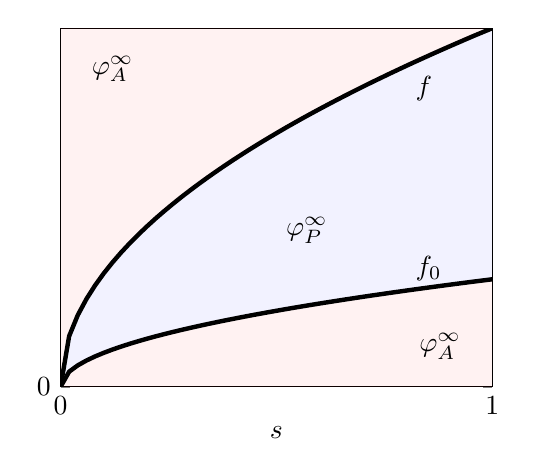
\begin{tikzpicture}[scale=0.8]
            \begin{axis}[xmin=0, xmax=1, ymin=0, ymax=1, samples at={0, 0.02, ..., 0.98, 1},
                    xtick={0, 1}, ytick={0}, xlabel={$s$}]
                \addplot[name path=f, ultra thick] {x^0.5};
                \addplot[name path=f0, ultra thick] {0.3 * x^0.5};
                \node[anchor=north west] at (axis cs: .8, .8^0.5) {$f$};
                \node[anchor=south west] at (axis cs: .8, .3*.8^0.5) {$f_0$};
                \path[name path=bottom] (axis cs:0,0) -- (axis cs:1,0);
                \path[name path=top] (axis cs:0,1) -- (axis cs:1,1);

                \addplot [fill=blue, fill opacity=0.05] fill between [of=f and f0];
                \addplot [fill=red, fill opacity=0.05] fill between [of=f and top];
                \addplot [fill=red, fill opacity=0.05] fill between [of=f0 and bottom];

                \node[anchor=north west, align=left] at (axis cs: .05, .95) {$\varphi_A^\infty$};
                \node[anchor=south east, align=left] at (axis cs: .95, .05) {$\varphi_A^\infty$};
                \node[anchor=north west, align=right] at (axis cs: .5, .5) {$\varphi_P^\infty$};
            \end{axis}
        \end{tikzpicture}
        \caption{Fringe can achieve relatively little without $P$}
    \end{subfigure}
    \begin{subfigure}[b]{0.45\textwidth}
        \centering
        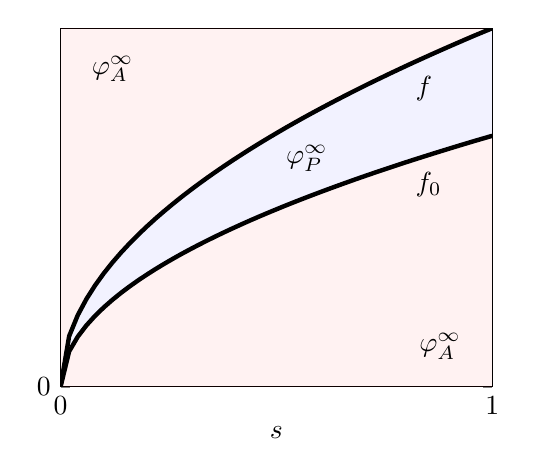
\begin{tikzpicture}[scale=0.8]
            \begin{axis}[xmin=0, xmax=1, ymin=0, ymax=1, samples at={0, 0.02, ..., 0.98, 1},
                    xtick={0, 1}, ytick={0}, xlabel={$s$}]
                \addplot[name path=f, ultra thick] {x^0.5};
                \addplot[name path=f0, ultra thick] {0.7 * x^0.5};
                \node[anchor=north west] at (axis cs: .8, .8^0.5) {$f$};
                \node[anchor=north west] at (axis cs: .8, .7*.8^0.5) {$f_0$};
                \path[name path=bottom] (axis cs:0,0) -- (axis cs:1,0);
                \path[name path=top] (axis cs:0,1) -- (axis cs:1,1);

                \addplot [fill=blue, fill opacity=0.05] fill between [of=f and f0];
                \addplot [fill=red, fill opacity=0.05] fill between [of=f and top];
                \addplot [fill=red, fill opacity=0.05] fill between [of=f0 and bottom];

                \node[anchor=north west, align=left] at (axis cs: .05, .95) {$\varphi_A^\infty$};
                \node[anchor=south east, align=left] at (axis cs: .95, .05) {$\varphi_A^\infty$};
                \node[anchor=north west, align=right] at (axis cs: .5, .7) {$\varphi_P^\infty$};
            \end{axis}
        \end{tikzpicture}
        \caption{Fringe can achieve relatively more without $P$}
    \end{subfigure}
    \caption{Distribution of value between player $P$ (blue) and the fringe (red)}
    \label{fig:non_indispensable}
\end{figure}


\section{Many-sided case}
\label{sec:many_sided}

Up until this point, we have only considered games with a single type of small player.
Now imagine that, in addition to player $P$, there are $L$ types of smaller players: $\{A^l_1, \dots, A^l_n\}$ where $1 \leq l \leq L$.
As before, assume that $P$ is necessary for any coalition to have a positive value, and the small players are identical to each other \emph{within their types}.
Formally, the game in coalitional form is now the following: the set of players is $N = \{P, A^1_1, \dots, A^1_n, \dots, A^L_1, \dots, A^L_n\}$ and the characteristic function is
\begin{align*}
    v(S) = \begin{cases}
        0                                                & \text{if } P \notin S \\
        f\left(\frac{n_{A^1}(S)}{n}, \dots, \frac{n_{A^L}(S)}{n}\right) & \text{otherwise}.
    \end{cases}
\end{align*}

A prominent interpretation of the two-sided version of this model would be a platform marketplace with a set of sellers and a set of buyers, where all three sides possess some amount of bargaining power.
However, player $P$ does not have to be in the ``middle'' of the transactions for this framework to be applicable.
For example, it also captures the situation of a single upstream producer, a large number of downstream firms, and a similarly large number of customers, as long as both the customers and the downstream firms can participate in the bargaining process.\footnote{
    A setting where these assumptions might be plausible is, for example, the new car market with a car producer, a number of independent dealerships, and customers who might engage in some form of negotiation.
}
Or, following \textcite{stole1996intra}, it could also be used to model bargaining between a firm and multiple types of workers.

Let us follow the pattern from the previous sections.
Start by characterizing conditions for monotonicity and superadditivity to support the bargaining interpretation and the formation of the grand coalition.
It is easy to see that the conditions are the straightforward analogues of those from the one-sided case.
\begin{proposition}
    The game $(N, v)$ is monotone and superadditive if and only if $f$ is increasing in all of its arguments.
\end{proposition}

In the next subsections, I will first examine random order values, and then two important special cases: the Shapley value and the weighted value.

% \subsection{Shapley value}

% Let us obtain formulas for the values of the three types of players.
% It turns out that the limits of the Shapley-values (as $n \to \infty$) are still analytically tractable, and they also have a neat interpretation.
% \begin{proposition}
%     Let $f$ be continuous everywhere on $[0, 1]^L$.
%     Then,
%     \begin{align*}
%         \varphi_P^\infty & = \int_0^1 f(t, \dots, t) \dt                                 \\
%         \varphi_{A^l}^\infty & = \int_0^1 t \partial_l f(t, \dots, t) \dt.
%     \end{align*}
% \end{proposition}

% As the previous proposition shows, the value of each kind of player depends on their expected marginal contribution, i.e. the partial derivatives of $f$.
% Consequently, the value of the grand coalition can be decomposed into the Shapley-values of its members the following way:
% \begin{align*}
%     f(1, \dots, 1) = \underbrace{\int_0^1 f(t, \dots, t) \dt}_{\text{ player } P} + \sum_{l=1}^L \underbrace{\int_0^1 t \partial_l f(t, \dots, t) \dt}_{\text{players } A^ll}.
% \end{align*}
% This formulation makes it clear that values are intimately related to the marginal contributions of the players, captured by the partial derivatives of $f$ in the case of the various fringe players.

% One surprising element of the result is that one only has to integrate over the diagonal of the support  of $f$, and the value does not depend on off-diagonal parts of the $f$ fucntion.
% The intuition for that relies on a law-of-large-numbers-type reasoning.
% If the number of fringe players is large, then it is very unlikely that, after a random ordering, their proportion is too different on any interval.
% Consequently, when taking the expectation over all orderings, those with very unequal numbers of the various types have little impact on it.


\subsection{Random order values}

Let us start by establishing the analog of \cref{prop:one_sided_general} for the many-sided case.
\begin{proposition}
    \label{prop:many_sided_general}
    Let $f$ be continuous on $[0, 1]^L$. Furthermore, let us denote the random vector of the proportions of the various types of fringe players before $P$ as $X_n$:
    \begin{align*}
        X_n = \left( \frac{n_{A_1}(\mathcal{P}_P)}{n}, \dots, \frac{n_{A_L}(\mathcal{P}_P)}{n} \right).
    \end{align*}
    Assume that $X_n \xrightarrow[]{d} X$ with cdf $G_X(t_1, \dots, t_L)$ and (if exists) pdf $g(t_1, \dots, t_L)$.
    Then
    \begin{align*}
        \varphi_P^\infty = \lim_{n \to \infty} \varphi_P^n &= \int_0^1 \dots \int_0^1 f(t_1, \dots, t_L) \dG(t_1, \dots t_L) \\
        &= \int_0^1\dots \int_0^1 g(t) f(t_1, \dots, t_L) \dt_1 \dots \dt_L,
    \end{align*}
    with the last equality holding if $X$ is a continuous random variable.
\end{proposition}

While the above proposition is very general in terms of permutation probabilities, it is not very tractable in practice, as one has to integrate over the entire unit hypercube.
It would be much more convenient, if one only had to be concerned with a one-dimensional manifold within the hypercube instead.
It turns out, that for a couple of important cases (namely, the Shapley value and the weighted value) it is indeed the case.

Let us start by establishing a general result, after which I will show that the Shapley value and the weighted value are special cases of it.

\begin{lemma}
    % TODO: check notation!
    \label{lem:many_sided_manifold}
    Assume that $X_n \xrightarrow[]{d} X$ where $X$ is a degenerate distribution in the following sense: $\exists \, a_l: [0, 1] \to [0, 1], l = 1, \dots, L$, such that
    \begin{align*}
        X = (a_1(\xi), \dots, a_L(\xi)),
    \end{align*}
    where $\xi$ is a random variable on $[0, 1]$ with cdf $H(s)$.
    In words, the whole probability mass is concentrated on the manifold $(a_1(s), \dots a_L(s)), t \in [0, 1]$.
    Then
    \begin{align*}
        \varphi_P^\infty = \lim_{n \to \infty} \varphi_P^n &= \int_0^1 f(a_1(s), \dots a_L(s)) \mathrm{d}H(s).
    \end{align*}
    Furthermore, if $f$'s partial derivatives exist on $\{(a_1(t), \dots, a_L(t)) : t \in [0, 1]\}$ the value of fringe $l$ has the following limit:
    \begin{align*}
        \varphi_{A^l}^\infty = \lim_{n \to \infty} \varphi_{A^l}^n &= \int_0^1 H(s) a_l'(s) \partial_l f(a_1(s), \dots a_L(s)) \ds.        
    \end{align*}
\end{lemma}

The lemma above states, that -- if its assumptions are satisfied -- one only has to be concerned with just a tiny fraction of the production function $f$.
Namely, we only need to know how the function behaves on the set $\{(a_1(t), \dots, a_L(t)) : t \in [0, 1]\} \subset [0, 1]^L$.\footnote{
    For the fringe players, we also need the partial derivatives.
    Therefore, technically, the behavior of $f$ on some arbitrarily small neighborhood of the set also matters.
}
This result is essentially a generalization of the diagonal formula from \textcite{aumann2015values} or \textcite{stole1996intra} to the case where permutation probabilities are not uniform.
The intuition behind it is the same: if the number of fringe players is large, then it is very unlikely that, after a random ordering, their proportion is very different from \emph{what it should be}.
The main difference is that, in this case, the ``what it should be'' part is not uniform, but rather given by the $a_l$ functions.

In the remainder of this section, I will show that the Shapley value satisfy the assumptions of the above lemma, and thus the limit of those values can be expressed as an integral over a one-dimensional path.

\subsection{Shapley-value}

Now let us turn our attention to the Shapley-value.
As mentioned before, due to the uniformity of the permutation probabilities, we get a diagonal formula in this case.
\Cref{prop:many_sided_shapley} establishes this result formally.

\begin{proposition}
    \label{prop:many_sided_shapley}
    Let $f$ be continuous on $[0, 1]^L$.
    Then,
    \begin{align*}
        \varphi_P^\infty & = \int_0^1 f(t, \dots, t) \dt
    \end{align*}
    and
    \begin{align*}
        \varphi_{A^l}^\infty = \int_0^1 t \partial_l f(t, \dots, t) \dt.
    \end{align*}
\end{proposition}

As displayed on \cref{fig:many_sided_shapley}, The value of player $P$ is the integral of $f$ over the diagonal of the unit hypercube.\footnote{
    \textcite{stole1996intra} also obtain this expression for the limiting case of their bargaining game.
    The proof of this proposition demonstrates a way to obtain it as a limit of the Shapley value of the finite games.
}
Furthermore, this result also demonstrates how the rest of the value is divided amongst the fringe players.
Namely, those having higher marginal contributions along the diagonal get a larger share of the value.

\begin{figure}
    \centering
    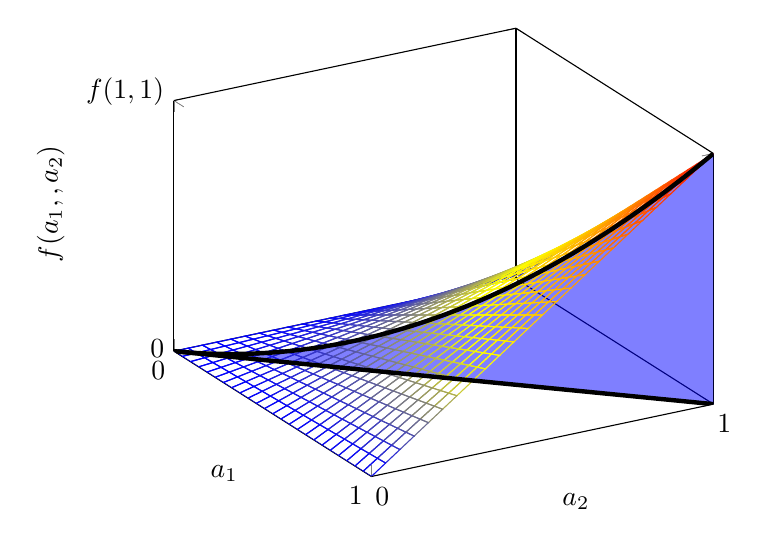
\begin{tikzpicture}
        \begin{axis}[
            xlabel={$a_1$}, ylabel={$a_2$}, zlabel={$f(a_1,, a_2)$},
            domain=0:1, y domain=0:1,
            zmin=0, zmax=1,
            xtick={0, 1}, ytick={0, 1}, ztick={0, 1},
            zticklabels={0, {$f(1, 1)$}}, % use the literal expression as a label
            view={60}{30}
        ]
            % plot the function
            \addplot3[surf, shader=flat, draw=none, name path=f, fill opacity=0] {x*y};
            % highlight the diagonal
            \addplot3[black, name path=diagonal, ultra thick, domain=0:1, samples=100, samples y=0] ({x}, {x}, {0});
            \addplot3[black, name path=f_diagonal, ultra thick, domain=0:1, samples=100, samples y=0] ({x}, {x}, {x^2});
            \addplot[blue, fill opacity=0.5] fill between[of=diagonal and f_diagonal];
        \end{axis}
    \end{tikzpicture}
    \caption{Illustration of the Shapley value in the case of two types of fringe players. The blue area corresponds to the value of the platform (with a scaling factor of $\sqrt{2}$ to account for the length of the diagonal)}
    \label{fig:many_sided_shapley}
\end{figure}


\subsection{Weighted value}

Let us now examine the weighted value in the multi-sided case.
The set of players and the characteristic function are the same as in the previous section, but players have the following weights: player $P$ has weight $\lambda_P$, while players $A^l_i$ have weight $\lambda_l$.
I will show, that as with the Shapley-value, the limit of the weighted value can also be expressed as an integral over a one-dimensional path.
However, this path is not the diagonal of the unit hypercube, and depends on the ratio of the fringe players' weights.

\begin{proposition}
    \label{prop:many_sided_weighted}
    Let $f$ be continuous on $[0, 1]^L$.
    Then,
    \begin{align*}
        \varphi_P^\infty & = \int_0^1 \lambda_P t^{\lambda_P - 1} f(t^{\lambda_1}, \dots, t^{\lambda^L}) \dt
    \end{align*}
    and
    \begin{align*}
        \varphi_{A^l}^\infty & = \int_0^1 t^{\lambda_P} \lambda_l t^{\lambda_l - 1} \partial_l f(t^{\lambda_1}, \dots, t^{\lambda^L}) \dt.
    \end{align*}
\end{proposition}

The intuition is the following.
A higher weight for a player means that it has a higher chance of being relatively late in a random permutation.
Therefore, conditional on $s$ proportion of the fringe coming before $P$, the various types' proportions do not reflect their population shares ($1/L$).
For any $s \in (0, 1)$, the proportion of fringe players with a higher weight is lower than their population share, while the proportion of fringe players with a lower weight is higher than their population share.
\Cref{fig:many_sided_weighted} illustrates this phenomenon in the case of two types of fringe players.

Finally, player $P$'s probability of coming after $s$ proportion of the fringe is also not uniform, but rather influenced by the relationship between its own and the fringe players' weights.
Therefore, the integral is not taken with respect to the uniform distribution, but rather one resembling that of \cref{prop:one_sided_weighted}.
The result is the following: when the big player has a higher weight, its chances of being relatively late in the ordering are higher, and thus -- due to $f$ being monotone increasing -- its value is higher.
The following, simple corollary formalizes this idea.

\begin{figure}
    \centering
    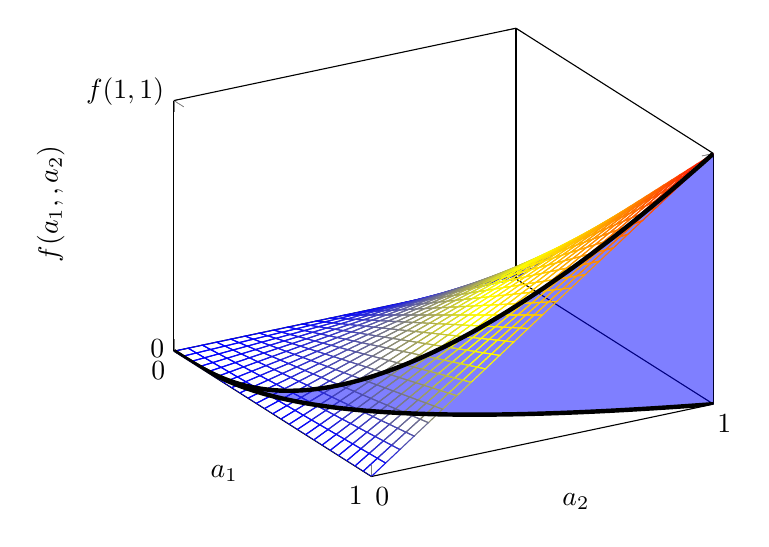
\begin{tikzpicture}
        \begin{axis}[
            xlabel={$a_1$}, ylabel={$a_2$}, zlabel={$f(a_1,, a_2)$},
            domain=0:1, y domain=0:1,
            zmin=0, zmax=1,
            xtick={0, 1}, ytick={0, 1}, ztick={0, 1},
            zticklabels={0, {$f(1, 1)$}}, % use the literal expression as a label
            view={60}{30}
        ]
            % plot the function
            \addplot3[surf, shader=flat, draw=none, name path=f, fill opacity=0] {x*y};
            % highlight the diagonal
            \addplot3[black, name path=diagonal, ultra thick, domain=0:1, samples=100, samples y=0] ({x}, {x^3}, {0});
            \addplot3[black, name path=f_diagonal, ultra thick, domain=0:1, samples=100, samples y=0] ({x}, {x^3}, {x^4});
            \addplot[blue, fill opacity=0.5] fill between[of=diagonal and f_diagonal];
        \end{axis}
    \end{tikzpicture}
    \caption{Illustration of the weighted value in the case of two types of fringe players. Players of type $A^2$ have a higher weight than those of type $A^1$, thus the integral is not taken over the diagonal. The blue area corresponds to the value of the platform (the area have to be scaled so that the length of the path integrated over is one)}
    \label{fig:many_sided_weighted}
\end{figure}

\begin{corollary}
    \label{cor:platform_value_multiple_sides_weighted}
    $\varphi_P^\infty$ is increasing in $\lambda_P$ unless $f$ is constant.
\end{corollary}


\section{Example application}

In this section I will apply the results of the previous sections to a simple model of two-sided platforms.
I follow the modelling approach of the monopoly platform case in \textcite{armstrong2006competition}, with a few extensions.
There are two major departures from the original model.
First, and most importantly, instead of letting the platform choose entry fees, I assume that they are the result of a bargaining process, and the outcomes are described by the weighted value.
Second, instead of assuming that each player's utility is linear in the number of the other side's players, I allow for more general (power) functions, which lets me capture the substitutability of the two sides.

\subsection{Model}

Imagine a two-sided market with a continuum of players on both sides.
Furthermore, assume that there is a single platform that connects the two sides.
The utility that a player on side $i$ derives from participating in the market is an increasing function\footnote{
    \textcite{armstrong2006competition} -- along with much of the literature on two-sided markets \parencite[e.g.][]{rochet2003platform,hagiu2006pricing} -- assumes that the utility of a player is linear in the number of players on the other side.
    Using a more general function allows me to model different degrees of network effects.
} of the number of players on the other side ($n_j$), minus the entry fee charged by the platform ($p_i$):
\begin{align*}
    u_i = \alpha_i n_j ^ {\gamma_i} - p_i,
\end{align*}
where $\alpha \geq 0$ and $\gamma > 0$ determine the strength and shape of the network effects, respectively.

Following \textcite{armstrong2006competition}, let us also model player entry in a reduced form manner.
Assume that there is a continuum of potential entrants on both sides, and the number of actual entrants is an increasing function of the utility achieved after entering\footnote{
    One possible microfoundation of this is assuming some idiosyncratic entry cost for the players.
    Then, the number of entrants is the number of players for whom the utility of entering is higher than the entry cost.
}:
\begin{align*}
    n_i = \phi_i(u_i).
\end{align*}

Finally, let us assume that the platform can charge lump-sum entry fees to both sides.
These fees can also be negative, in which case they are interpreted as subsidies.
The platform's profit is the sum of entry fees, minus the cost of serving the entrants ($F_i$ for each entrant):
\begin{align*}
    \pi(n_1, n_2) = n_1 p_1 + n_2 p_2 - F_1 n_1 - F_2 n_2.
\end{align*}

I will consider two cases as to the timing and nature of the price-setting process, as well as a welfare-maximizing benchmark.
For the latter, I derive the entry fees that maximize social welfare, i.e. the sum of the utilities of the two sides plus the platform's profit.
After that, I will first consider a model analogous to that in \textcite{armstrong2006competition}, where the platform can unilaterally commit to any entry fees it wishes.
Finally, I consider a model in which entry fees are the result of a bargaining process in such a way that the resulting utilities and profits correspond to the various players' weighted values.

\subsection{Benchmark: welfare-maximizing entry fees}

Let us consider first what entry fees would maximize social welfare.
Instead of approaching this problem directly, let us rely on the following observation: if entry fees correspond to the externality that a player's entry imposes on the other side, then the resulting choices are welfare-maximizing.
In this specific case, there are two externalities to consider.
First, it costs the platform $F_i$ to serve an additional player on side $i$.
Second, the entry of a player on side $i$ increases the utility on side $j$ due to positive network effects.
Welfare is maximized when the price reflects the balance of these two  factors:
\begin{align*}
    p_i^* &= F_i - n_j \frac{\partial u_j}{\partial n_i} \\
          &= F_i - \alpha_j \gamma_j n_j n_i^{\gamma_j - 1}.
\end{align*}
As in \textcite{armstrong2006competition}, for any $\alpha_j > 0$ welfare-maximizing $F_i$ is below the platform's cost of serving player $i$.
Thus, the platform's profit would necessarily be negative.
It naturally cannot happen in the case when the platform sets the entry fees, or even the bargaining case.

As an immediate corollary, utilities in this case are given by
\begin{align*}
    u_i^* = \alpha_i n_j ^ {\gamma_i} + \alpha_j \gamma_j n_j n_i^{\gamma_j - 1} - F_i.
\end{align*}
Furthermore, the utility of type $i$ depends positively on both $\alpha_i$ (mechanically) and $\alpha_j$ (a stronger positive externality on the other players implies a lower entry fee and thus higher utility).
Finally, if $n_i \geq e^{-\frac{1}{\gamma_j}}$, then $u_i$ is also increasing in $\gamma_j$.
Both of the latter two effects are related to player $i$ being compensated for the positive externality it imposes on the other side.

\subsection{Platform sets prices unilaterally}

Now let us examine what happens when the platform sets the entry fees unilaterally.
First, rewrite the platform's profit as a function of utilities, rather than the number of entrants:
\begin{align*}
    \pi(u_1, u_2) = \phi_1(u_1) [\alpha_1 \phi_2(u_2) ^ {\gamma_1} - u_1 - F_1] + \phi_2(u_2) [\alpha_2 \phi_1(u_1) ^ {\gamma_2} - u_2 - F_2].
\end{align*}

Let us assume that the above expression is concave, and thus the first order conditions characterize its maximum.
Then, simply taking the partial derivatives with respect to $u_i$ yields the following condition for the optimal entry fees.
\begin{proposition}
    \label{prop:platform_unilateral}
    If the platform can set entry fees unilaterally, then optimal entry fees for side $i$ are characterized by
    \begin{align*}
        p_i^u &= F_i - \alpha_j \gamma_j n_j n_i^{\gamma_j - 1} + \frac{\phi_1(u_1)}{\phi'_1(u_1)} \\
              &= p_i^* + \frac{\phi_1(u_1)}{\phi'_1(u_1)}.
    \end{align*}
\end{proposition}

As one would expect, profit-maximizing entry fees are higher than welfare-maximizing ones.
In addition to the comparative statics of the welfare-maximizing case, the platform's entry fees also depend on the elasticity of entry.
When it is low, the platform will set a high entry fee, as the loss of entrants is small.

For ease of comparison with the bargaining case, let us also derive the utilities in this case:
\begin{align*}
    u_i^u = \alpha_i n_j ^ {\gamma_i} + \alpha_j \gamma_j n_j n_i^{\gamma_j - 1} - F_i - \frac{\phi_1(u_1)}{\phi'_1(u_1)}.
\end{align*}
Clearly, as equilibrium utilities must be smaller than in the welfare-maximizing case, due to $\phi_i$ being increasing, the number of entrants is also lower.

\subsection{Bargaining}

Finally, let us consider the case when the platform and the players bargain over the entry fees.
To do this, let us impose some structure on the timing of the game.
The idea is that even though the platform cannot commit to a specific entry fee structure anymore, it can commit to a bargaining process.
Specifically, it is able to commit to a bargaining weight for each side and itself: $\lambda_P, \lambda_1, \lambda_2$.

Then, the game proceeds as follows.
In the first period, the platform chooses $\lambda_P, \lambda_1$ and $\lambda_2$.
After that, potential antrants on both sides simultaneously decide whether to enter or not.
Finally, in the last period, the platform and the entrants bargain over the entry fees, and utilities are realized according to their weighted values.

Let us start by looking at the last period.
Assume that $n_1$ and $n_2$ players have decided to enter on sides $1$ and $2$, respectively.
Furthermore, assume that bargaining weights are $\lambda_1, \lambda_2$ and $\lambda_P$.

The characteristic function of the game takes a similar form to that in \cref{sec:many_sided}.
If the platform is not part of the coalition, then the value is zero.
Otherwise, it is simply the sum of the utilities of the two sides minus the cost of serving them.\footnote{
    The entry fees do not matter, as they are simply payments between coalition members, and thus do not affect the total value.
}
This value, as a function of the number of entrants, is
\begin{align*}
    w(n_1, n_2) = n_1 \alpha_1 n_2^{\gamma_1} + n_2 \alpha_2 n_1^{\gamma_2} - F_1 n_1 - F_2 n_2.
\end{align*}

The share received by each type of player is then easily established using \cref{prop:many_sided_weighted}.
\begin{proposition}
    \label{prop:platform_bargaining_last_period}
    Let $f(t_1, t_2) = w(t_1 n_1, t_2 n_2)$. Then the weighted values of the various sides are
    \begin{alignat*}{4}
        \varphi_P(n_1, n_2) &= \underbracket{\frac{\lambda_P}{\lambda_P + \lambda_1 + \lambda_2\gamma_1}}_{\coloneqq S_P^{b_1}} \alpha_1 n_1 n_2^{\gamma_1} &&+ \underbracket{\frac{\lambda_P}{\lambda_P + \lambda_2 + \lambda_1\gamma_2}}_{\coloneqq S_P^{b_2}} \alpha_2 n_2 n_1^{\gamma_2} &&- \underbracket{\frac{\lambda_P}{\lambda_P + \lambda_1}}_{\coloneqq S_P^{c_1}} n_1 F_1 &&- \underbracket{\frac{\lambda_P}{\lambda_P + \lambda_2}}_{\coloneqq S_P^{c_2}} n_2 F_2 \\
        \varphi_1(n_1, n_2) &= \underbracket{\frac{\lambda_1}{\lambda_P + \lambda_1 + \lambda_2\gamma_1}}_{\coloneqq S_1^{b_1}} \alpha_1 n_1 n_2^{\gamma_1} &&+ \underbracket{\frac{\lambda_1 \gamma_2}{\lambda_P + \lambda_2 + \lambda_1\gamma_2}}_{\coloneqq S_1^{b_2}}  \alpha_2 n_2 n_1^{\gamma_2} &&- \underbracket{\frac{\lambda_1}{\lambda_P + \lambda_1}}_{\coloneqq S_1^{c_1}} n_1 F_1 && \\
        \varphi_2(n_1, n_2) &= \underbracket{\frac{\lambda_2\gamma_1}{\lambda_P + \lambda_1 + \lambda_2\gamma_1}}_{\coloneqq S_2^{b_1}} \alpha_1 n_1 n_2^{\gamma_1} &&+ \underbracket{\frac{\lambda_2}{\lambda_P + \lambda_2 + \lambda_1\gamma_2}}_{\coloneqq S_2^{b_1}} \alpha_2 n_2 n_1^{\gamma_2} && &&- \underbracket{\frac{\lambda_2}{\lambda_P + \lambda_2}}_{\coloneqq S_2^{c_2}} n_2 F_2.
    \end{alignat*}
\end{proposition}

\section{Conclusions}

This paper proposed a new framework to think about the profit allocation in situations concerning a few large and a continuum of smaller players.
The results are especially relevant for upstream-downstream situations, platform settings, and two-sided markets.
The outcomes of the Shapley-value-based gain sharing rule generally concur with intuitive expectations, and the resulting formulas are more tractable than most explicit non-cooperative approaches.

% The illustrative model also highlights the strengths of this approach.
% Despite its simplicity, it highlights that the effects of vertical integration strongly depends on the substitutability of the downstream firms.
% In a time when upstream firms and platforms are increasingly seeking to sell directly to the consumers\footnote{
%     As some recent examples, consider the recent acquisition of Whole Foods by Amazon, Microsoft's ongoing efforts to buy Activision/Blizzard (a major video game publisher), or Tesla's or BMW's plans to sell cars directly without the help of dealerships.
% }
% , such results can be important for competition authorities.

There is a variety of ways in which this paper could be expanded or built upon.
On the theoretical side, a number of the assumptions, such as fringe agents achieving a zero payoff without the platform, could be relaxed,
Besides this, the convergence result for the weighted values could be strengthened if one could manage to show that any sequence along ever more refined partitions of the atomic players converges to the same limit \parencite[à la][]{fogelman1980asymptotic}.

A slightly different direction would be to consider other solution concepts from cooperative game theory in this specific setting.
One obvious candidate is the nucleolus, which shares many of the useful properties of the Shapley-value (it always exists and is unique).
Furthermore, it also has connections to bargaining theory due to it being contained in the core when the latter exists.

The possibilities for practical applications are no less interesting.
The proposed profit sharing framework could be embedded in a more applied model of some real-life setting.
For a step in this direction, see \textcite{stancsics2023hybrid}.

Finally, with time, the cooperative approach to profit distribution could become an almost drop-in alternative of the more usual, but in some sense more extreme assumptions about the bargaining process widely used in industrial organization models.


\appendix

\printbibliography

\section{Miscellaneous lemmas}

\begin{lemma}
    \label{lemma:log_convergence}
    Let 
    \begin{align*}
        \Delta_n(s) &= \frac{\log(s + 1/n) - \log(\lambda)}{n}, \\
        \Delta(s) &= \frac{1}{s}.
    \end{align*}
    Then $\Delta_n \xrightarrow[]{\mathrm{u}} \Delta$ uniformly on $[t, 1]$ for any $t > 0, \lambda > 0$.
\end{lemma}
\begin{proof}[Proof of \cref{lemma:log_convergence}]
    First, note that $\Delta_n$ and $\Delta$ are all continuous functions.
    Then, following the standard proof for $\frac{\mathrm{d}}{\mathrm{d}s}log(s) = \frac{1}{s}$ rewrite $\Delta_n(s)$ as
    \begin{align*}
        \Delta_n(s) &= \frac{\log(s + 1/n) - \log(\lambda)}{n} \\
        &= \log \left( 1 + \frac{1}{sn} \right) ^ n .
    \end{align*}
    It is well known that $\left( 1 + \frac{1}{sn} \right) ^ n$ is monotone increasing in $n$ and converges to $\exp (1/s)$.
    Therefore, the pointwise convergence of $\Delta_n(s) \to \Delta(s)$ is also monotone.

    Finally, by Dini's theorem, the monotone pointwise convergence of a sequence of continuous functions to a continuous function on a compact set implies uniform convergence on that set.
\end{proof}

\begin{lemma}
    \label{lemma:integral_convergence}
    Let $f_n, f: [a, b] -> \mathbb{R}$ be Riemann-integrable functions with $f_n \xrightarrow[]{\mathrm{u}} f$ uniformly.
    Then,
    \begin{align*}
        \lim_{n \to \infty} \frac{b-a}{n} \sum_{k=1}^n f_n \left( a + \frac{b-a}{n} \right) = \int_0^1 f(t) \dt.
    \end{align*}
\end{lemma}
\begin{proof}[Proof of \cref{lemma:integral_convergence}]
    \begin{align*}
        &\lim_{n \to \infty} \frac{b-a}{n} \sum_{k=1}^n f_n \left( a + \frac{b-a}{n} \right) \\
        &= \lim_{n \to \infty} \frac{b-a}{n} \left[ \sum_{k=1}^n f \left( a + \frac{b-a}{n} \right) + \sum_{k=1}^n \left( f_n \left( a + \frac{b-a}{n} \right) - f \left( a + \frac{b-a}{n} \right) \right) \right] \\
        &= \int_a^b f(t) \dt + \lim_{n \to \infty} \frac{b-a}{n}\sum_{k=1}^n \left( f_n \left( a + \frac{b-a}{n} \right) - f \left( a + \frac{b-a}{n} \right) \right) \\
        &\leq \int_a^b f(t) \dt + \lim_{n \to \infty} \frac{b-a}{n}\sum_{k=1}^n \left| f_n \left( a + \frac{b-a}{n} \right) - f \left( a + \frac{b-a}{n} \right) \right| \\
        &\leq \int_a^b f(t) \dt + \lim_{n \to \infty} \frac{b-a}{n}\sum_{k=1}^n \sup_{t \in [a, b]} \left| f_n(t) - f(t) \right| \\
        &= \int_a^b f(t) \dt + (b-a) \underbrace{\lim_{n \to \infty} \sup_{t \in [a, b]} \left| f_n(t) - f(t) \right|}_{=0 \text{ due to uniform convergence}} \\
        &= \int_a^b f(t) \dt
    \end{align*}
\end{proof}

\begin{lemma}
    \label{lem:convergence_to_manifold}
    Consider the random vector $X_n$ with values from $[0, 1]^L$.
    Let $S_n = \sum_l[X_n]_l / L$, with the cumulative distribution function $G_n(s)$.
    Assume that for every $s \in [0, 1]$, $X_n \mid n S_n = \lfloor ns \rfloor \xrightarrow[]{L^1} h(s)$ where $h(s)$ is some continuous function.
    Let $S_n \xrightarrow[]{d} S$.
    Then $X_n \xrightarrow[]{d} h(S)$.
\end{lemma}

\begin{proof}[Proof of \cref{lem:convergence_to_manifold}]
    We have to show that
    \begin{align*}
        \lim_{n \to \infty} \Pr(X_n \leq x) = \Pr(h(S) \leq x).
    \end{align*}
    for any $x$ where the cdf of $h(S)$ is continuous.

    Let us start by conditioning on $S_n$:
    \begin{align*}
        \Pr(X_n \leq x) = \int_0^1 \Pr(X_n \leq x \mid S_n = s) \dG_n(s).
    \end{align*}
    Now consider the following:
    \begin{align*}
        \lim_{n \to \infty} \left| \Pr(X_n \leq x) - \Pr(h(S) \leq x) \right| &= \lim_{n \to \infty} \left| \int_0^1 \Pr(X_n \leq x \mid S_n = s) \dG_n(s) - \Pr(h(S) \leq x) \right| \\
        &\leq \lim_{n \to \infty} \left| \int_0^1 \Pr(X_n \leq x \mid S_n = s) \dG_n(s) - \Pr(h(S_n) \leq x) \right| \\
        &+ \lim_{n \to \infty} \left| \Pr(h(S_n) \leq x) - \Pr(h(S) \leq x) \right|
    \end{align*}
    for all $x \in [0, 1]^L$.
    I will show that both limits on the right-hand side are zero.

    Let us start with the first term.
    \begin{align*}
        \lim_{n \to \infty} &\left| \int_0^1 \Pr(X_n \leq x \mid S_n = s) \dG_n(s) - \Pr(h(S_n) \leq x) \right| \\
        &= \lim_{n \to \infty} \left| \int_0^1 \Pr(X_n \leq x \mid S_n = s) \dG_n(s) - \int_0^1 \mathbf{1}[h(s) \leq s] \dG_n(s) \right| \\
        &= \lim_{n \to \infty} \left| \int_0^1 \Pr(X_n \leq x \mid S_n = s) - \mathbf{1}[h(s) \leq x] \dG_n(s) \right| \\
        &= \lim_{n \to \infty} \left| \int_0^1 \underbrace{\Pr(X_n \leq x \mid nS_n = \lfloor ns \rfloor) - \mathbf{1}[h(s) \leq x]}_{\coloneqq r(s)} \dG_n(s) \right| \\
        &\leq \lim_{n \to \infty} \int_0^1 \left| \Pr(X_n \leq x \mid nS_n = \lfloor ns \rfloor) - \mathbf{1}[h(s) \leq x] \right| \dG(s) \\
        &+ \lim_{n \to \infty} \left| \int_0^1 r(s) \dG_n(s) - \int_0^1 r(s) \dG(s) \right| \\
        &= 0.
    \end{align*}
    The first limit is zero because $X_n \mid n S_n = \lfloor ns \rfloor \xrightarrow[]{L^1} h(s)$.
    The second limit is zero because of the continuous mapping theorem, as $S_n \xrightarrow[]{p} S$ and $\Pr_S(s : r\text{ is not continuous at }s)= 0$.

    All that remains is to show that the second term is also zero.
    This simply follows from the continuous mapping theorem, as $f$ is continuous and $S_n \xrightarrow[]{d} S$.
\end{proof}


\section{Proofs of propositions in the main text}
\label{sec:proofs}

\begin{proof}[Proof of \cref{prop:monotone}]
    Monotonicity is evident.
    For superadditivity, note that for any coalitions $S_1, s_2$ such that $S_1 \cap s_2 = \emptyset$, $P \notin S_1$ or $P \notin s_2$.
    WLOG assume it is the latter, therefore $v(S_2) = 0$.
    As a result, $v(S_1) + v(S_2) = v(S_1) \leq v(S_1 \cup S_2)$ holds if and only if $(N, v)$ is monotone.
\end{proof}

\begin{proof}[Proof of \cref{prop:one_sided_general}]
    First, observe that $f$ is continuous on the compact set $[0, 1]$, and is therefore also bounded.
    Furthermore,
    \begin{align*}
        \varphi_P^n = \frac{1}{n+1} \sum_{k=0}^n \Pr(|\mathcal{P}_P| / n = k) f(k/n) = \E[X_n].
    \end{align*}
    As $f$ is continuous and bounded, and $X_n \xrightarrow[]{d} X$, by Portmanteau's lemma, $\E[f(X_n)] \to \E[f(X)]$.
    Putting it together,
    \begin{align*}
        \lim_{n \to \infty} \varphi_P^n &= \frac{1}{n+1} \sum_{k=0}^n \Pr(|\mathcal{P}_P| / n = k) f(k/n) \\
        &= \lim_{n \to \infty} \E[X_n] \\
        &= \E[X] \\
        &= \int_0^1 f(t) \dG(t).
    \end{align*}
    Furthermore, if $G$ is differentiable, then
    \begin{align*}
        \int_0^1 f(t) \dG(t) = \int_0^1 g(t) f(t) \dt.
    \end{align*}
\end{proof}

\begin{proof}[Proof of \cref{prop:one_sided}]
    Let $R$ denote a permutation of the set of players ($N$).
    Additionally, let us denote the players preceding $i$ by $\mathcal{P}_i^R$.
    The value of player $P$ is their expected marginal contribution averaged over all permutations of $N$:
    \begin{align*}
        \varphi_P^n = \frac{1}{(n+1)!} \sum_R v(\mathcal{P}_P^R \cup \{i\}) - v(\mathcal{P}_P^R)
    \end{align*}
    First, note that $v(\mathcal{P}_P^R) = 0$ for any permutation, as no coalition can achieve a positive value without player $P$.
    Furthermore, using the fact that all agents of type $A$ are identical implies that $v(\mathcal{P}_P^R \cup \{i\})$ only depends on the number of agents in the coalition.
    More precisely, 
    \begin{align*}
        v(\mathcal{P}_P^R \cup \{i\}) = f(n_A(\mathcal{P}_P^R \cup \{i\}) / n) = f(|\mathcal{P}_P^R| / n).
    \end{align*}
    Finally, the set of permutations in which $k$ number of players precede $P$ is independent of $n$, i.e.
    \begin{align*}
        \{R \mid |\mathcal{P}_P^R| = k\} = n! \quad \forall\, k.
    \end{align*}
    Putting all the above together, the value of player $P$ can be expressed as
    \begin{align*}
        \varphi_P^n &= \frac{1}{(n+1)!} \sum_{k=0}^n n! f(k / n) \\
        &= \frac{1}{n+1} \sum_{k=0}^n f(k / n) \\
        &= \frac{n}{n+1} \underbrace{\frac{1}{n} \sum_{k=0}^{n-1} f(k / n)}_{=S_n} + \frac{1}{n+1} f(1).
    \end{align*}
    $S_n$ are just the left Riemann-sums of function $f$ on the interval $[0, 1]$.
    Therefore, if $f$ is continuous (and thus Riemann-integrable), then $S_n \to \int_0^1 f(t)$, and thus
    \begin{align*}
        \lim_{n \to \infty} \varphi_P^n &= \lim_{n \to \infty} \frac{1}{n+1} \sum_{k=1}^n f(k / n) \\
        &= \lim_{n \to \infty}\underbrace{\frac{n}{n+1}}_{\to 1} \frac{1}{n} \sum_{k=0}^{n-1} f(k / n) + \underbrace{\frac{1}{n+1} f(1)}_{\to 0} \\
        &= \int_0^1 f(t) \dt .
    \end{align*}
\end{proof}

\begin{proof}[Proof of Corollary \ref{cor:fringe_value}]
    The first equality comes from the efficiency of the Shapley-value.
    The values of all players sum up to $f(1)$ for all $n \in \mathbb{N}$, therefore
    \begin{align*}
        \lim_{n \to \infty} \sum_{i=1}^n \varphi_{A_i}^n = \lim_{n \to \infty} (1 - \varphi_P^n ) = 1 - \int_0^1 f(t).
    \end{align*}
    The second can be obtained by integration by parts:
    \begin{align*}
        \int_0^1 t f'(t) \dt = tf(t) \mid_0^1 - \int_0^1 f(t) \dt = f(1) - \int_0^1 f(t) \dt
    \end{align*}
\end{proof}

\begin{proof}[Proof of \cref{lem:entry_distr}] %\textcolor{red}{(Might have to fix sum indices)} \\
    The probability of $P$ having at most fraction $t$ of the other players before itself is
    \begin{align*}
        \Pr(X_n \leq nt) &= \Pr(X_n \leq nt ) \\
        &= \prod_{j = nt + 1}^n \frac{j}{j + \lambda} \\
        &= \exp \Bigg( \underbrace{\sum_{j = nt + 1}^n \log(j) - \log(j+\lambda)}_{\equiv S_n} \Bigg).
    \end{align*}
    Taking limits,
    \begin{align*}
        \lim_{n \to \infty} S_n &= \lim_{n \to \infty} \sum_{j = nt + 1}^n \log(j) - \log(j+\lambda) \\
        &= \lim_{n \to \infty} \sum_{i = 1}^{n - nt} \log(nt + i) - \log(nt + i + \lambda) \\
        &= \lim_{n \to \infty} \frac{1}{n - nt} \sum_{i = 1}^{n - nt} \frac{\log \left( t + \frac{i}{n - nt} \right) - \log \left( t + \frac{i}{n - nt} + \frac{\lambda}{n - nt} \right)}{1 / (n - nt)}
    \end{align*}
    Let
    \begin{align*}
        \Delta_n(s) = \frac{\log \left( s \right) - \log \left( s + \frac{\lambda}{n - nt} \right)}{1 / (n - nt)}
    \end{align*}
    By lemma \ref{lemma:log_convergence}, 
    \begin{align*}
        \Delta_n \xrightarrow[]{\mathrm{u}} \lambda \frac{\mathrm{d}}{\mathrm{d}s}log(s) = -\frac{\lambda}{s}
    \end{align*}
    on the compact interval $[t, 1]$ for any $t > 0$ ($\xrightarrow[]{\mathrm{u}}$ denotes uniform convergence).
    
    Then, by lemma \ref{lemma:integral_convergence}, we have that
    \begin{align*}
        \lim_{n \to \infty} S_n &= \lim_{n \to \infty} \frac{1}{n-nt} \sum_{i=1}^{n-nt} \Delta_n \left( t + \frac{i}{n - nt} \right) \\
        &= \int_t^1 (\lim_{n \to \infty} \Delta_n)(s) \ds \\
        &= \int_t^1 \lim_{n \to \infty} -\frac{\lambda}{s} \ds \\
        &= \lambda \log{t}
    \end{align*}

    Substituting $\lim_{n \to \infty} S_n$ into the original equation yields
    \begin{align*}
        \lim \Pr \left( \frac{X_n}{n} \leq t \right) &= \exp \Bigg( \lim_{n \to \infty} \sum_{j = nt + 1}^n \log(j) - \log(j+\lambda) \Bigg) \\
        &= \exp(\lambda \log(t)) \\
        &= t^\lambda.
    \end{align*}

    For $t=0$, simply observe that %\textcolor{red}{Have to elaborate on this}
    \begin{align*}
        \lim_{n \to \infty} \prod_{j = 1}^n \frac{j}{j + \lambda} = 0 = 0^\lambda.
    \end{align*}
\end{proof}

\begin{proof}[Proof of Corollary \ref{cor:fringe_value_2}]
    If $f$ is monotone increasing, then $f(0) \leq \int_0^1 f(t) \dt \leq f(1)$.
    The inequalities become strict if $f$ is not constant on the whole interval.
\end{proof}

\begin{proof}[Proof of \cref{prop:one_sided_weighted}]
    The weighted value of player $P$ is its expected contribution across all permutations, with each permutation weighted by its probability of occurring.
    \begin{align*}
        \varphi_P^{n, \lambda} = \sum_R \Pr(R) [v(\mathcal{P}_P^R \cup \{i\}) - v(\mathcal{P}_P^R)]
    \end{align*}
    As before, using the fact that fringe players are identical, this can be rephrased as
    \begin{align*}
        \varphi_P^{n, \lambda} &= \sum_{k=0}^n \Pr(R) f(k/n) \\
        &= \E[f(X_n / n)]
    \end{align*}
    where $X_n$ is defined as above.
    $f$ is continuous, and therefore bounded on the compact set $[0, 1]$.
    As a consequence, $\frac{X_n}{n} \xrightarrow[]{d} X$ implies $\E[f(X_n / n)] \to \E[f(X)]$, which in turn gives
    \begin{align*}
        \lim_{n \to \infty} \varphi_P^{n, \lambda} &= \lim_{n \to \infty} \E[f(X_n / n)] \\
        &= \E[f(X)] \\
        &= \int_0^1 f(t) \dG(t) \\
        &= \int_0^1 g(t)f(t) \dt
    \end{align*}
    where $G(t)$ and $g(t)$ are the cdf and pdf of X, respectively.
\end{proof}

\begin{proof}[Proof of Corollary \ref{cor:platform_value_weighted}]
    Let $X$ and $X'$ be random variables with cdfs $G_X = t^\lambda$ and $G_{X'}t^{\lambda'}$, respectively.
    For any $\lambda < \lambda'$, $t^\lambda > t^{\lambda'} \forall t \in [0, 1]$, meaning that $X'$ first-order stochastically dominates $X'$.
    As a result, for any monotonically increasing $f$,
    \begin{align*}
        \int_0^1 g_X(t)f(t) \dt = \E[f(X)] \leq \E[f(X')] = \int_0^1 g_{X'}(t)f(t)
    \end{align*}
    with strict inequality unless $f$ is constant almost everywhere.
    As $f$ is continuous, the latter is equivalent to $f$ being constant on the whole $[0, 1]$ interval.
\end{proof}

\begin{proof}[Proof of Corollary \ref{cor:paltform_value_weighted_2}]
    As $\lambda \to 0$, $X$ converges to the degenerate random variable $X_0$ for which $\Pr(X_0 = 0) = 1$.
    As a consequence, the expected value of $f(X)$ converges to $\E[f(X_0)] = f(0)$.
    $\lim_{\lambda \to \infty} \varphi^{\infty, \lambda}_P = f(1)$ can be shown along the same lines.
\end{proof}

\begin{proof}[Proof of \cref{prop:multiple_platforms}]
    \label{prop:one_sided_multiple}
    First, let us rewrite the expected marginal contribution of player $P_i$ in the following way:
    \begin{align*}
        \varphi_{P_i}^{n, m} &= \frac{1}{(n+m)!} \sum_R v(\mathcal{P}_{P_i}^R \cup \{i\}) - v(\mathcal{P}_{P_i}^R) \\
        &= \frac{1}{(n+m)!} \left[ \sum_{\{R | n_P(\mathcal{P}_{P_i}^R = 0)\}} \left[v(\mathcal{P}_{P_i}^R \cup \{i\}) - v(\mathcal{P}_{P_i}^R)\right] + \sum_{\{R | n_P(\mathcal{P}_{P_i}^R > 0)\}} \left[v(\mathcal{P}_{P_i}^R \cup \{i\}) - v(\mathcal{P}_{P_i}^R)\right] \right]
    \end{align*}
    Next, make use of the fact that the marginal contribution of a platform is zero if another platform is already present, and only depends on the number of fringe firms otherwise.
    \begin{align*}
        \varphi_{P_i}^{n, m} &= \frac{1}{(n+m)!} \sum_{\{R | n_P(\mathcal{P}_{P_i}^R = 0)\}} f (\mathcal{P}_{A}^R / n) \\
        &= \frac{1}{(n+m)!} \sum_{k=0}^n |\{R | n_A(\mathcal{P}^R_{P_i} = k) \text{ and } n_P(\mathcal{P}^R_{P_i} = 0)\}| f(k/n)
    \end{align*}
    Finally, notice that, while the permutations with $k$ fringe agents before $P_i$ does not depend on $k$, amongst those, the number of permutations with no platform before $P_i$ does depend on it.
    In particular,
    \begin{align*}
        |\{R | n_A(\mathcal{P}^R_{P_i} = k) \text{ and } n_P(\mathcal{P}^R_{P_i} = 0)\}| &= \frac{n!(n+m-k-1)!}{(n-k)!}
    \end{align*}
    and
    \begin{align*}
        \varphi_{P_i}^{n, m} &= \sum_{k=0}^n \frac{n!(n+m-k-1)!}{(n+m)!(n-k)!} f(k/n) \\
        &= \sum_{k=0}^n \frac{(n-k+1)(n-k+2) \dots (n-k+m-1)}{(n+1)(n+2) \dots (n+m)} f(k/n) \\
        &= \frac{1}{n+1}\sum_{k=0}^n \underbrace{\frac{(n(1-k/n)+1)(n(1-k/n)+2) \dots (n(1-k/n)+m-1)}{(n+2) \dots (n+m)} f(k/n)}_{S_n}
    \end{align*}
    For any $t = k/n \in [0, 1]$, 
    \begin{align*}
        S_n(t) \to (1-t)^{m-1}f(t) \equiv S(t).
    \end{align*}
    Furthermore, it is simple to verify that this convergence is uniform, and that $S_n$ and $S$ are all continuous functions.
    By Dini's theorem, the former properties imply that $S_n \xrightarrow[]{\mathrm{u}} S$ uniformly on $[0, 1]$.

    The conclusion of the proof is similar to that of proposition \ref{prop:one_sided}:
    \begin{align*}
        \lim_{n \to \infty} \varphi_{P_i}^{n, m} &= \lim_{n \to \infty} \underbrace{\frac{n}{n+1}}_{\to 1} \sum_{k=0}^{n-1} S_k(k/n) + \underbrace{\frac{1}{1+n}S(1)}_{\to 0} \\
        &= \lim_{n \to \infty} \sum_{k=0}^{n-1} S_k(k/n) \\
        &= \int_0^1 (1-t)^{m-1} f(t) \dt
    \end{align*}
    with the last equality supported by lemma \ref{lemma:integral_convergence}.
\end{proof}

\begin{proof}[Proof of Corollary \ref{cor:multiple_platforms}]
    The allocation is efficient for all $n \in \mathbb{N}$, therefore efficient in the limit, as well.
    The second equality can be obtained by integration by parts.
\end{proof}

\begin{proof}[Proof of Corollary \ref{cor:multiple_platforms_2}] (Assuming $f$ is continuously differentiable) %\textcolor{red}{(Assuming $f$ is continuously differentiable -- will have to relax this)}
    $f'(t)$ is non-negative, so $[1 - (1-t)^m] f'(t)$ is increasing in $m$ $\forall t \in [0, 1]$.
    As a consequence, $\varphi_A^{n, \infty}$ is also increasing in $m$ if $f'(t)$ is positive on some interval or, $f(t)$ is not constant.
    Conversely, $\varphi_{P}^{\infty, m} = 1 - \varphi_{A}^{\infty, m}$ is decreasing in $m$.
\end{proof}

\begin{proof}[Proof of \cref{prop:many_sided_general}]
    The proof mirrors that of \cref{prop:one_sided_general}.
    First, note that the random order value can be expressed as follows:
    \begin{align*}
        \varphi_P^n &= \sum_{k_1=0}^n \dots \sum_{k_L=0}^n \Pr(n_{A_1}(\mathcal{P}_P) = k_1, \dots, n_{A_L}(\mathcal{P}_P) = k_L) f\left(\frac{k_1}{n}, \dots, \frac{k_L}{n}\right) \\
        &= \sum_{k_1=0}^n \dots \sum_{k_L=0}^n \Pr(n X_n = (k_1, \dots, k_L)) f\left(\frac{k_1}{n}, \dots, \frac{k_L}{n}\right) \\
        &= \sum_{k_1=0}^n \dots \sum_{k_L=0}^n \Pr \left( X_n = \left(\frac{k_1}{n}, \dots, \frac{k_L}{n}\right) \right) f \left(\frac{k_1}{n}, \dots, \frac{k_L}{n}\right) \\
        &= \E[f(X_n)].
    \end{align*}
    Furthermore, as $f$ is continuous (and therefore bounded on $[0, 1]^L$), and $X_n \xrightarrow[]{d} X$, by Portmanteau's lemma, $\E[f(X_n)] \to \E[f(X)]$.
    Putting it together,
    \begin{align*}
        \lim_{n \to \infty} \varphi_P^n &= \lim_{n \to \infty} \E[f(X_n)] \\
        &= \E[f(X)] \\
        &= \int_0^1 \dots \int_0^1 f(t_1, \dots, t_L) \dG(t_1, \dots t_L).
    \end{align*}
    Finally, if $X$ is a continuous random variable, then
    \begin{align*}
        \int_0^1 \dots \int_0^1 f(t_1, \dots, t_L) \dG(t_1, \dots t_L) = \int_0^1\dots \int_0^1 g(t_1, \dots, t_L) f(t_1, \dots, t_L) \dt_1 \dots \dt_L.
    \end{align*}
\end{proof}

\begin{proof}[Proof of \cref{lem:many_sided_manifold}]
    Just like in the proof of \cref{prop:many_sided_general}, the random order value can be expressed as follows:
    \begin{align*}
        \varphi_P^n &= \E[f(X_n)].
    \end{align*}
    Furthermore, as $f$ is continuous and bounded on $[0, 1]^L$, and $X_n \xrightarrow[]{d} X$, by Portmanteau's lemma, $\E[f(X_n)] \to \E[f(X)]$.
    Therefore,
    \begin{align*}
        \lim_{n \to \infty} \varphi_P^n &= \lim_{n \to \infty} \E[f(X_n)] \\
        &= \E[f(X)] \\
        &= \E[f(a_1(\xi), \dots, a_L(\xi))] \\
        &= \int_0^1 f(a_1(s), \dots a_L(s)) \mathrm{d}H(s).
    \end{align*}
\end{proof}

\begin{proof}[Proof of \cref{prop:many_sided_shapley}]
    Let us show than $X_n$ converges in distribution to the degenerate random variable $X = (U, \dots, U)$, where $U$ is uniformly distributed on $[0, 1]$.

    Let us first define the random variable $S_n = \sum_l[X_n]_l / L$, the total number of small players placed before $P$.
    Also, define $h(s) = (s, \dots, s)$.
    Now let us look at the conditional distribution $n X_n | n L S_n = k$.
    As all permutations have equal probability, this is the same as picking $kL$ firms from the set $N \setminus \{P\}$ without replacement.
    The numbers of each type in this sample will follow a multinomial distribution with $kL$ trials, $L$ events and probabilities $1/L$.

    Let us now show that $\Pr(X_n < x \mid S_n = s) \xrightarrow[]{\mathrm{u}} \mathbf{1}[(s, \dots, s) \leq x]$ on $s \in \mathrm{supp}(S_n)$.

    First, observe that
    \begin{align*}
        [\E(n X_n | nS_n = \lfloor ns \rfloor)]_l &= \lfloor ns \rfloor, \\
        [\Var(n X_n | nS_n = \lfloor ns \rfloor)]_l &= \lfloor ns \rfloor \frac{L-1}{L}
    \end{align*}
    for all $\quad l = 1, \dots, L$.
    Consequently,
    \begin{align*}
        [\E(X_n | nS_n = \lfloor ns \rfloor)]_l &= \frac{\lfloor ns \rfloor}{n}, \\
        [\Var(X_n | nS_n = \lfloor ns \rfloor)]_l &= \frac{\lfloor ns \rfloor}{n^2} \frac{L-1}{L}
    \end{align*}
    for all $\quad l = 1, \dots, L$.

    Notice that, as $n \to \infty$, $[\Var(X_n | nS_n = \lfloor ns \rfloor)]_l \to 0$.
    Furthermore, $\E(X_n | nS_n = \lfloor ns \rfloor) \to h(s)$.
    Thus, for any $s \in [0, 1], X_n | nS_n = \lfloor ns \rfloor \xrightarrow[]{L^2} h(s)$.

    Let us now turn to the random variable $S_n$.
    Observe that because the probability of each permutation is the same, player $P$ has the same probability of being in any position.
    In other words, $S_n$ follows a uniform distribution on $0, \frac{1}{nL}, \frac{2}{nL} \dots, 1$.
    Consequently, $S_n$ converges in distribution to the uniform distribution $U[0, 1]$.

    I have now shown that the assumptions of \cref{lem:convergence_to_manifold} are satisfied.
    % TODO

    Then, by \cref{lem:many_sided_manifold}, the Shapley-value is
    \begin{align*}
        \varphi_P^\infty & = \int_0^1 f(t, \dots, t) \dt.
    \end{align*}

\end{proof}

\begin{proof}[Proof of \cref{prop:many_sided_weighted}]
    The proof uses the same approach as that of \cref{prop:many_sided_shapley}.
    I will show that $X_n \xrightarrow[]{d} h(\xi)$, where $h(s) = (s^{\lambda_1}, \dots, s^{\lambda_L})$, and $\xi$ is a random variable with cdf $G(s) = s^{\lambda_P}$, and then rely on \cref{lem:many_sided_manifold}.

    

\end{proof}

\end{document}
